%%%%%%%%%%%%%%%%%%%%%%%%%%%%%%%%%%%%%%%%%%%%%%%%%%%%%%%%%%%%%%%%%%%%%%%%%%%
\chapter{Étude de la viabilité commerciale}
\label{Chapitre_3}
%%%%%%%%%%%%%%%%%%%%%%%%%%%%%%%%%%%%%%%%%%%%%%%%%%%%%%%%%%%%%%%%%%%%%%%%%%%

\textit{Démontrer la viabilité commerciale d'une solution ne se limite pas à identifier un besoin ou à décrire un produit : cela exige de prouver que l'offre est monétisable, scalable et défendable dans un contexte concurrentiel donné. Ce chapitre construit la stratégie commerciale de Vocallia selon une chaîne logique unique où chaque décision découle de la précédente et prépare la suivante : la segmentation identifie à qui vendre en premier ; le positionnement formule pourquoi ces clients choisiront Vocallia ; le Value Proposition Canvas vérifie que le produit répond précisément à leurs douleurs ; l'analyse SWOT fixe les priorités d'exécution ; le modèle économique organise la capture de valeur ; le marketing mix et le go-to-market en déploient les leviers opérationnels ; la tarification, les unit economics et les projections financières en démontrent la rentabilité. L'ensemble constitue un plan d'action commercial directement opérationnel, destiné à guider les premières années d'activité de Vocallia.}

%%%%%%%%%%%%%%%%%%%%%%%%%%%%%%%%%%%%%%%%%%%%%%%%%%%%%%%%%%%%%%%%%%%%%%%%%%%
\section{Segmentation et ciblage}
\label{section3.1}
%%%%%%%%%%%%%%%%%%%%%%%%%%%%%%%%%%%%%%%%%%%%%%%%%%%%%%%%%%%%%%%%%%%%%%%%%%%

La segmentation est l'acte fondateur de toute stratégie commerciale : elle détermine à qui l'on s'adresse, dans quel ordre, et avec quels arguments. Pour Vocallia, cette décision est d'autant plus critique que le marché e-commerce tunisien est hétérogène --- il mêle des structures formalisées aux boutiques informelles sur réseaux sociaux, des marchands numériquement matures à ceux qui découvrent les outils digitaux. En phase d'amorçage, se tromper de cible initiale ne ralentit pas la croissance : cela tue le projet. Concentrer les ressources sur le segment où la douleur est la plus aiguë, la capacité à payer la plus immédiate et le cycle de vente le plus court est une condition de survie.

%%%%%%%%%%%%%%%%%%%%%%%%%%%%%%%%%%%%%%%%%%%%%%%%%%%%%%%%%%%%%%%%%%%%%%%%%%%
\subsection{Segmentation multicritères}
\label{section3.1.1}
%%%%%%%%%%%%%%%%%%%%%%%%%%%%%%%%%%%%%%%%%%%%%%%%%%%%%%%%%%%%%%%%%%%%%%%%%%%

La segmentation de Vocallia repose sur une approche multicritères combinant des dimensions opérationnelles, comportementales et économiques. Elle s'appuie sur les données collectées lors de l'étude exploratoire terrain (22 répondants, avril 2025) et sur l'analyse du marché e-commerce tunisien (BCT, 2024). Six critères structurants ont été retenus, chacun constituant un filtre discriminant pour évaluer l'intensité du besoin, la capacité d'adoption et la solvabilité de chaque segment.

\begin{table}[H]
\centering
\caption{Segmentation multicritères --- Vocallia (2025)}
\vspace{4pt}
\begin{tabularx}{\textwidth}{|>{\raggedright\arraybackslash}p{3cm}|>{\raggedright\arraybackslash}X|>{\raggedright\arraybackslash}X|>{\raggedright\arraybackslash}X|}
\hline
\textbf{Critère} & \textbf{Segment A \newline Cible prioritaire} & \textbf{Segment B \newline Cible secondaire} & \textbf{Segment C \newline Hors cible initiale} \\
\hline
Volume commandes/jour & $>$ 15 commandes & 6 à 15 commandes & $<$ 5 commandes \\
\hline
Mode de paiement dominant & Cash on delivery (COD) exclusif & COD et prépaiement mixte & Prépaiement majoritaire \\
\hline
Ancienneté de la boutique & 3 ans et plus & 1 à 3 ans & Moins de 1 an \\
\hline
Gestion des appels & Gérant ou employé dédié & Gérant seul, sans ressource & Externalisé ou inexistant \\
\hline
Appétence digitale & Utilise déjà des outils SaaS & Utilisateur partiel, curieux & Faible maturité digitale \\
\hline
Budget mensuel estimé & 100--300 DT/mois & 50--100 DT/mois & $<$ 50 DT/mois \\
\hline
Intensité du besoin & \textbf{Critique} --- le problème est coûteux et quotidien & \textbf{Réelle} --- le problème est présent mais supportable & \textbf{Faible} --- pas de friction opérationnelle identifiée \\
\hline
Priorité commerciale & \textbf{Haute} & Moyenne & \textbf{Absente au lancement} \\
\hline
\end{tabularx}
\end{table}

La matrice de priorisation (figure~\ref{fig:matrice_segments}) synthétise visuellement cette hiérarchisation en croisant l'intensité du besoin avec la capacité à payer de chaque segment.

\begin{figure}[H]
\centering
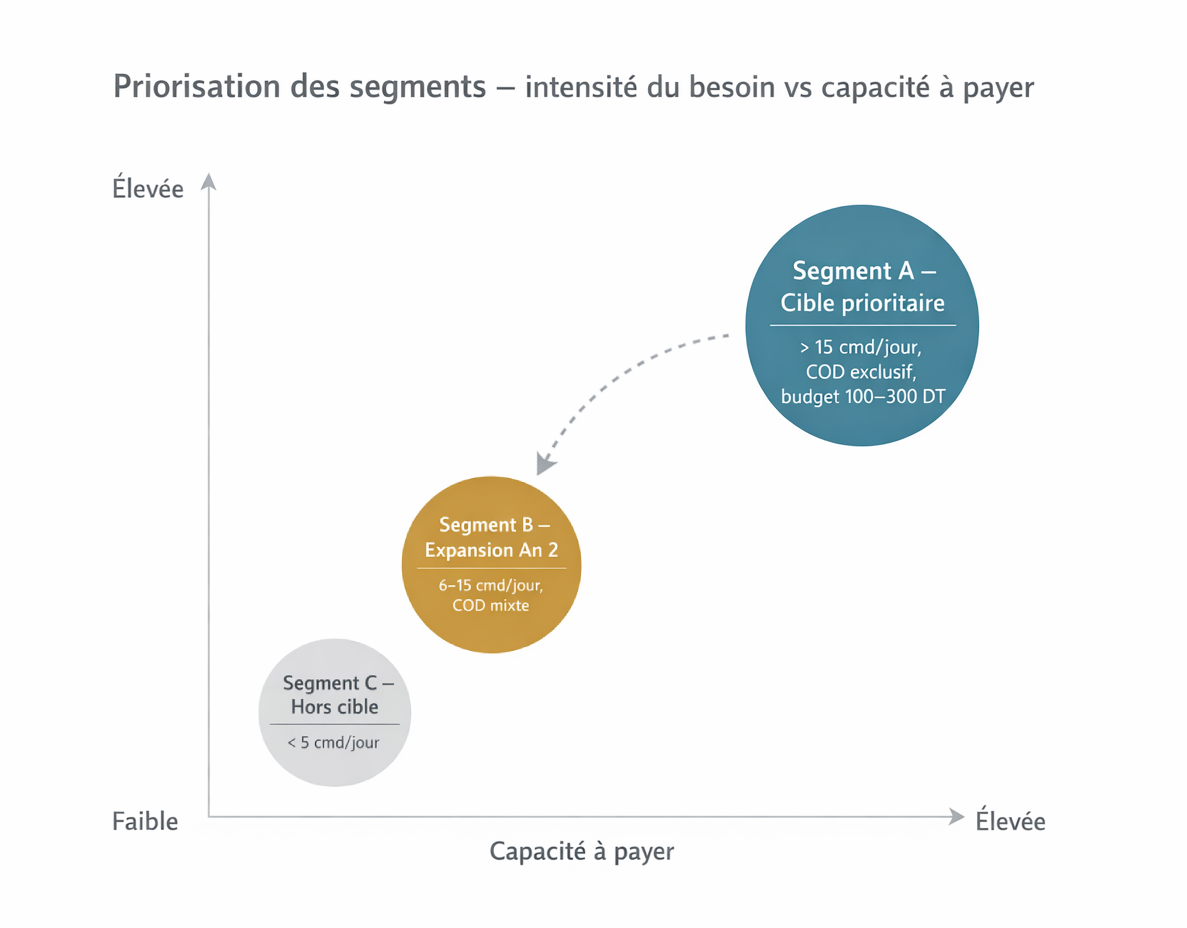
\includegraphics[width=0.82\textwidth]{figures/matrice_priorisation_segments.png}
\caption{Priorisation des segments --- intensité du besoin vs capacité à payer}
\label{fig:matrice_segments}
\end{figure}

\noindent\textbf{Lecture stratégique de la segmentation.} Le Segment A est le seul où Vocallia génère de la valeur dès le premier mois, avec un risque commercial minimal et un cycle de vente court. Le Segment B représente un réservoir de croissance naturel à moyen terme : ces marchands basculeront lorsque les résultats du Segment A fourniront les preuves sociales nécessaires. Le Segment C est délibérément exclu au lancement : le coût d'acquisition y serait disproportionné, le risque de churn élevé, et l'impact sur les métriques SaaS destructeur dans une phase où chaque point de crédibilité compte.

Cette hiérarchisation conditionne l'intégralité de la stratégie qui suit : le positionnement sera formulé pour le Segment A, la proposition de valeur calibrée sur ses douleurs, le pricing ancré dans sa zone de confort budgétaire, et le go-to-market optimisé pour son cycle de décision.

%%%%%%%%%%%%%%%%%%%%%%%%%%%%%%%%%%%%%%%%%%%%%%%%%%%%%%%%%%%%%%%%%%%%%%%%%%%
\subsection{Personas commerciaux}
\label{section3.1.2}
%%%%%%%%%%%%%%%%%%%%%%%%%%%%%%%%%%%%%%%%%%%%%%%%%%%%%%%%%%%%%%%%%%%%%%%%%%%

Au-delà des segments, la stratégie commerciale est orientée par deux personas représentatifs, construits à partir des données qualitatives de l'étude terrain. Ces profils ne sont pas des archétypes théoriques : ils incarnent des réalités opérationnelles documentées, et servent de guide aussi bien pour la conception produit que pour les argumentaires de vente.

\begin{figure}[H]
\centering
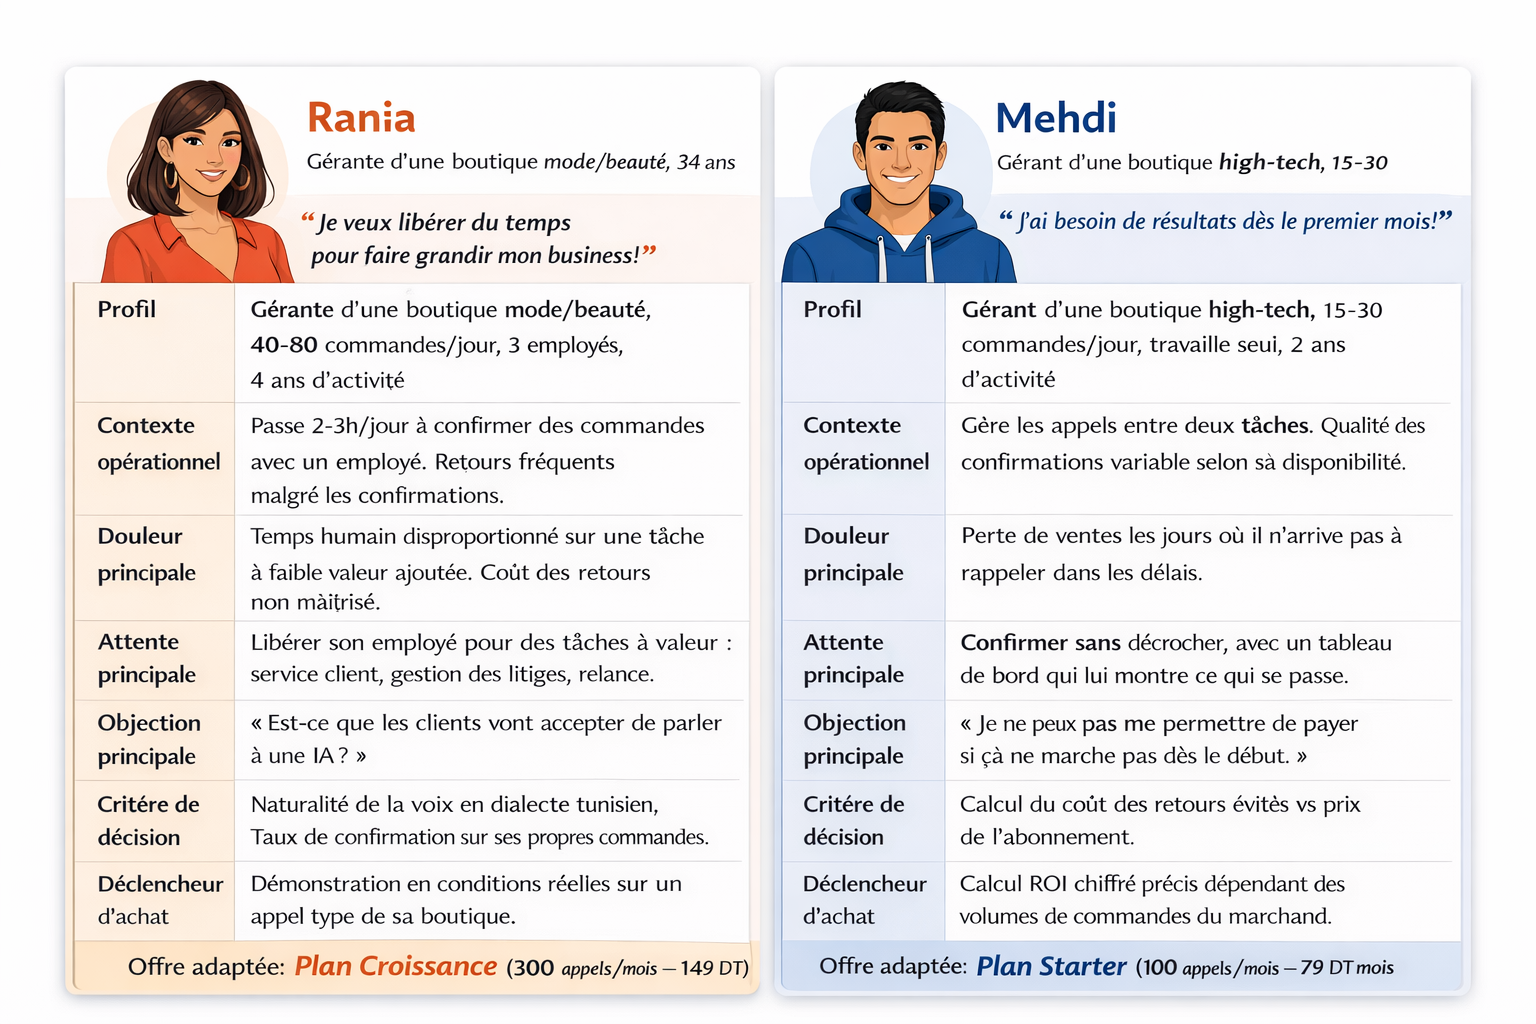
\includegraphics[width=\textwidth]{figures/personas_vocallia.png}
\caption{Personas commerciaux --- Vocallia}
\label{fig:personas}
\end{figure}

\noindent\textbf{Interprétation stratégique des personas.} Les deux profils structurent des approches commerciales distinctes, mais convergent vers un même impératif : la preuve par le résultat. Avec Rania, le levier de conversion est la libération de capacité opérationnelle et la réduction mesurable des coûts --- un argument qui se traduit directement en économies chiffrées sur le dashboard. Avec Mehdi, le levier est la tranquillité opérationnelle et la rapidité du gain perçu, condition non négociable pour déclencher l'achat chez un dirigeant qui investit sur ses fonds propres. Dans les deux cas, le moment de bascule du cycle de vente est le même : l'écoute d'un appel réel en dialecte tunisien, validé comme le déclencheur de conversion le plus puissant lors de la phase Muvaka. Ce constat oriente directement le positionnement : Vocallia doit se vendre comme une performance opérationnelle audible et mesurable, pas comme une promesse technologique.

%%%%%%%%%%%%%%%%%%%%%%%%%%%%%%%%%%%%%%%%%%%%%%%%%%%%%%%%%%%%%%%%%%%%%%%%%%%
\section{Positionnement stratégique}
\label{section3.2}
%%%%%%%%%%%%%%%%%%%%%%%%%%%%%%%%%%%%%%%%%%%%%%%%%%%%%%%%%%%%%%%%%%%%%%%%%%%

Le positionnement est la décision stratégique la plus structurante du plan commercial : il détermine comment la marque veut être perçue, par rapport à qui, et sur quelle promesse irréductible. La segmentation a identifié le Segment A comme cible prioritaire ; les personas ont révélé que le critère de décision est la performance opérationnelle mesurable, pas l'innovation technologique. Le positionnement de Vocallia en découle directement. Dans un marché où aucun concurrent local direct n'existe encore, ce positionnement n'est pas défensif --- il est fondateur. L'enjeu n'est pas de se différencier d'un concurrent, mais de définir la catégorie avant que quiconque ne tente de l'occuper.

\medskip
\noindent\textbf{Énoncé de positionnement.} \textit{Vocallia est la première infrastructure locale d'automatisation vocale intelligente pour les e-commerçants tunisiens : elle confirme vos commandes en dialecte tunisien, 24h/24, à un coût marginal faible, avec une traçabilité complète --- pour que vous confirmiez plus, perdiez moins, et vous concentriez sur ce qui fait vraiment croître votre activité.}

\medskip
Ce positionnement repose sur trois piliers stratégiques distincts et défendables à moyen terme (figure~\ref{fig:positionnement_piliers}).

\begin{figure}[H]
\centering
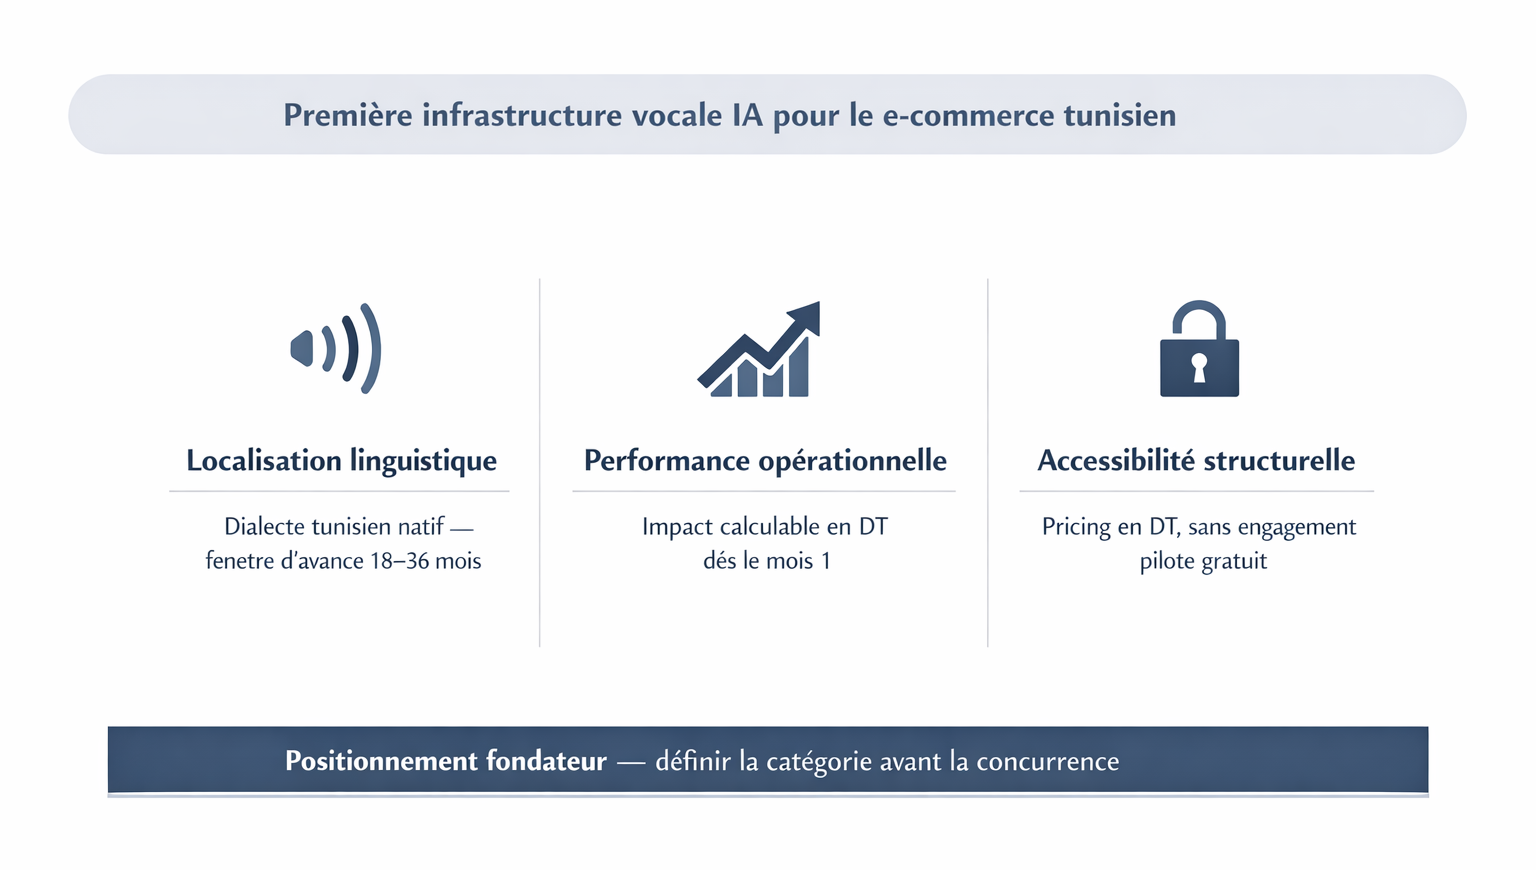
\includegraphics[width=\textwidth]{figures/positionnement_3piliers.png}
\caption{Positionnement stratégique Vocallia --- trois piliers défendables}
\label{fig:positionnement_piliers}
\end{figure}

La \textbf{localisation linguistique} --- maîtrise du dialecte tunisien (darija) et du code-switching arabe/français --- constitue une barrière à l'entrée que les acteurs globaux (Bland.ai, Vapi.ai, Retell AI) ne peuvent franchir sans un investissement local spécifique, coûteux et long. Cette barrière offre une fenêtre d'avance de 18 à 36 mois, suffisante pour construire une base de clients, un corpus de données d'appels locales et une réputation terrain irremplaçables.

L'\textbf{orientation performance opérationnelle} positionne Vocallia non comme une technologie, mais comme un levier de performance dont l'impact est calculable en dinars dès le premier mois d'usage. Cette posture --- partenaire de croissance plutôt que fournisseur technologique --- est décisive pour des PME dont le budget est contraint et dont la patience pour un outil sans résultat visible est nulle.

L'\textbf{accessibilité structurelle} --- pricing en dinars tunisiens, sans engagement long terme, avec un pilote gratuit --- élimine les trois principaux freins à l'adoption identifiés sur le terrain : le risque financier, la méfiance envers un outil nouveau, et l'absence de référence locale. Ces éléments ne sont pas des concessions --- ils font partie intégrante de la promesse de marque et structurent le modèle d'acquisition décrit dans les sections suivantes.

\medskip
Ce positionnement à trois piliers formule une promesse. La section suivante vérifie, à travers le Value Proposition Canvas, que cette promesse est effectivement tenue par le produit : chaque pilier doit correspondre à une douleur documentée, et chaque fonctionnalité doit y répondre avec précision.

%%%%%%%%%%%%%%%%%%%%%%%%%%%%%%%%%%%%%%%%%%%%%%%%%%%%%%%%%%%%%%%%%%%%%%%%%%%
\section{Proposition de valeur --- Value Proposition Canvas}
\label{section3.3}
%%%%%%%%%%%%%%%%%%%%%%%%%%%%%%%%%%%%%%%%%%%%%%%%%%%%%%%%%%%%%%%%%%%%%%%%%%%

Le Value Proposition Canvas (Osterwalder, Pigneur, Bernarda \& Smith, 2014) met en correspondance explicite le profil du client avec la carte de valeur du produit. Il sert ici de test de cohérence : le positionnement promet localisation, performance et accessibilité --- le VPC vérifie que le produit délivre sur ces trois axes. Toute fonctionnalité sans douleur correspondante serait superflue ; toute promesse sans ancrage terrain serait un risque commercial.

%%%%%%%%%%%%%%%%%%%%%%%%%%%%%%%%%%%%%%%%%%%%%%%%%%%%%%%%%%%%%%%%%%%%%%%%%%%
\subsection{Profil client}
\label{section3.3.1}
%%%%%%%%%%%%%%%%%%%%%%%%%%%%%%%%%%%%%%%%%%%%%%%%%%%%%%%%%%%%%%%%%%%%%%%%%%%

\begin{table}[H]
\centering
\caption{Profil client --- Value Proposition Canvas Vocallia}
\vspace{4pt}
\begin{tabularx}{\textwidth}{|>{\raggedright\arraybackslash}p{2.5cm}|>{\raggedright\arraybackslash}X|>{\raggedright\arraybackslash}X|}
\hline
\textbf{Dimension} & \textbf{Description détaillée} & \textbf{Preuve terrain} \\
\hline
\textbf{Jobs à accomplir} & Confirmer les commandes avant expédition. Gérer les demandes d'information client (délai, suivi). Maintenir la relation client pendant la livraison. Piloter le taux de retour. & Structurel : 84~\% des transactions en COD (BCT, 2024). Besoin quotidien, non délégable sans risque. \\
\hline
\textbf{Douleurs (Pains)} & Temps excessif mobilisé sur des appels répétitifs à faible valeur. Clients injoignables générant des retours coûteux. Annulations post-confirmation non anticipées. Qualité variable des échanges humains. Absence totale de données sur les raisons d'annulation. & 77,3~\% ont perdu des opportunités de vente (étude terrain, avr. 2025). Coût logistique d'un retour estimé à 12 DT (transport aller-retour). \\
\hline
\textbf{Gains attendus (Gains)} & Augmenter le taux de confirmation sans recruter. Libérer du temps pour des tâches à valeur. Réduire le taux de retour. Disposer d'un tableau de bord sur les annulations. Scaler l'activité sans augmenter les coûts fixes. & 90,9~\% se déclarent prêts à tester un pilote (étude terrain, avr. 2025). \\
\hline
\end{tabularx}
\end{table}

%%%%%%%%%%%%%%%%%%%%%%%%%%%%%%%%%%%%%%%%%%%%%%%%%%%%%%%%%%%%%%%%%%%%%%%%%%%
\subsection{Carte de valeur Vocallia}
\label{section3.3.2}
%%%%%%%%%%%%%%%%%%%%%%%%%%%%%%%%%%%%%%%%%%%%%%%%%%%%%%%%%%%%%%%%%%%%%%%%%%%

\begin{table}[H]
\centering
\caption{Carte de valeur --- Value Proposition Canvas Vocallia}
\vspace{4pt}
\begin{tabularx}{\textwidth}{|>{\raggedright\arraybackslash}p{2.5cm}|>{\raggedright\arraybackslash}X|>{\raggedright\arraybackslash}X|}
\hline
\textbf{Dimension} & \textbf{Réponse Vocallia} & \textbf{Alignement avec le profil client} \\
\hline
\textbf{Produits et services} & Agent vocal IA sortant, dialecte tunisien natif, disponible 24h/24, tableau de bord temps réel, transcriptions d'appels, intégration CRM via webhook, fallback humain automatique. & Couvre l'intégralité des Jobs identifiés sans intervention humaine constante. \\
\hline
\textbf{Analgésiques (Pain relievers)} & Appels automatiques $\rightarrow$ temps libéré. Script standardisé $\rightarrow$ qualité constante. Détection d'annulation $\rightarrow$ alerte immédiate. Fallback humain $\rightarrow$ aucun blocage conversationnel. Consentement vocal $\rightarrow$ conformité INPDP. & Adresse directement et précisément les 5 douleurs documentées sur le terrain. \\
\hline
\textbf{Créateurs de gains (Gain creators)} & Plus de commandes confirmées $=$ plus de CA. Réduction du taux de retour $=$ économies logistiques mesurables. Données sur les raisons d'annulation $=$ pilotage commercial. Scalabilité sans recrutement $=$ levier de croissance. & Répond aux 4 gains prioritaires exprimés par les personas Rania et Mehdi. \\
\hline
\end{tabularx}
\end{table}

%%%%%%%%%%%%%%%%%%%%%%%%%%%%%%%%%%%%%%%%%%%%%%%%%%%%%%%%%%%%%%%%%%%%%%%%%%%
\subsection{Représentation visuelle du Value Proposition Canvas}
\label{section3.3.3}
%%%%%%%%%%%%%%%%%%%%%%%%%%%%%%%%%%%%%%%%%%%%%%%%%%%%%%%%%%%%%%%%%%%%%%%%%%%

\begin{figure}[H]
\centering
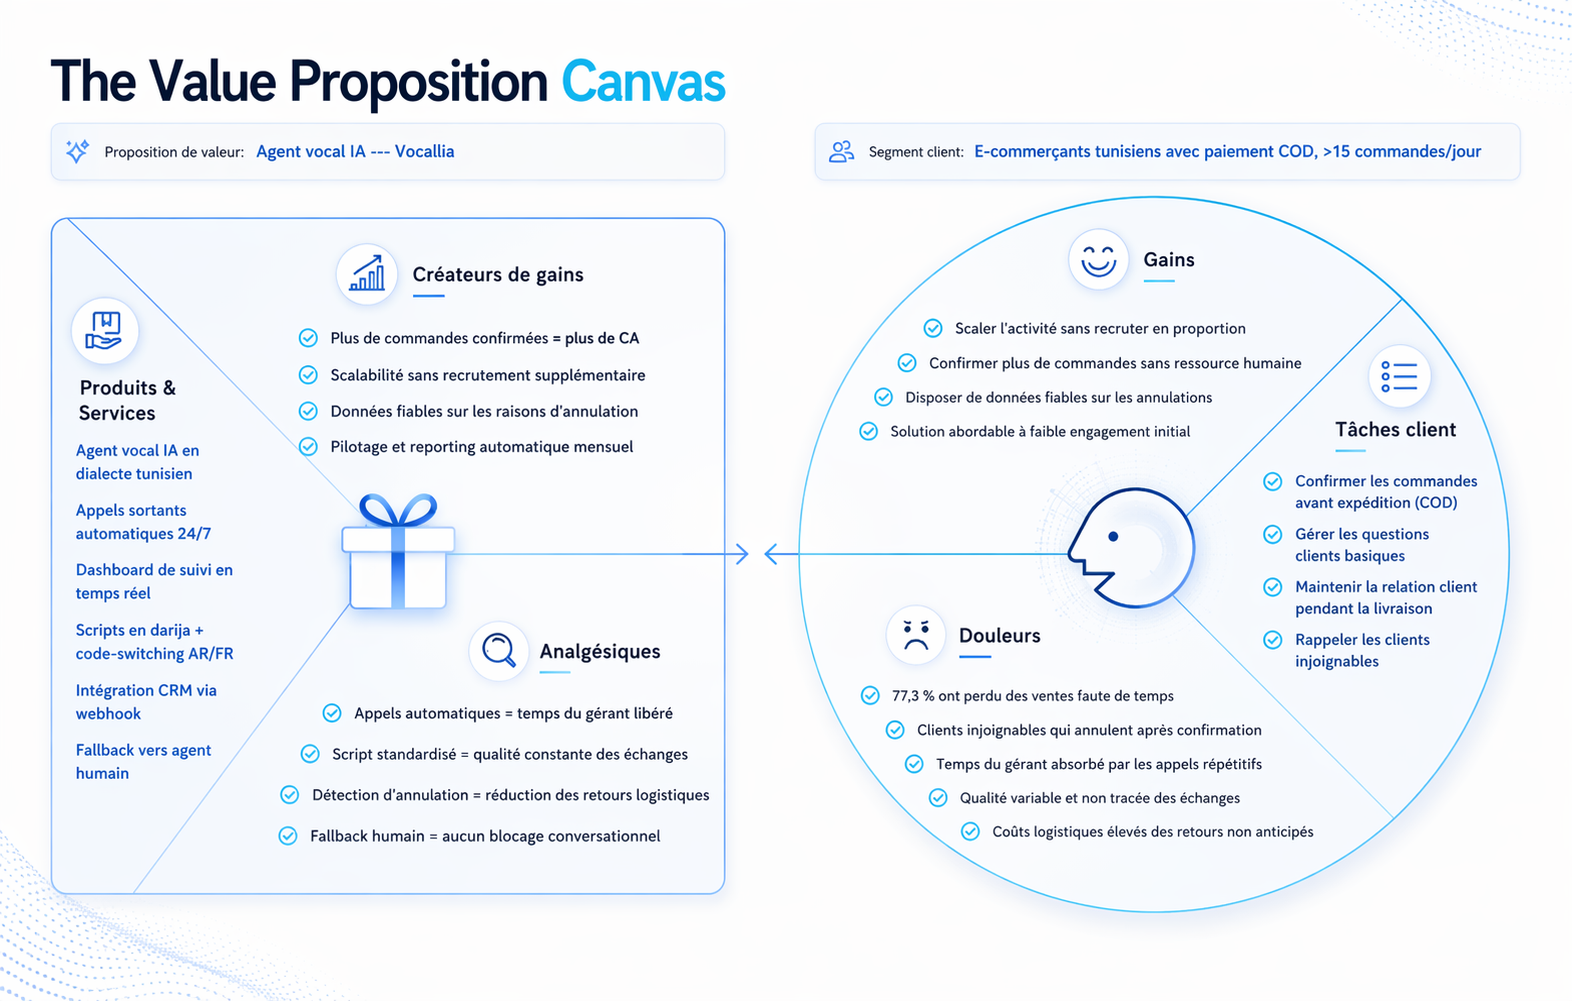
\includegraphics[width=\textwidth]{figures/value_proposition_canvas.png}
\caption{Value Proposition Canvas --- Vocallia (2025)}
\label{fig:vpc}
\end{figure}


\begin{tcolorbox}[colback=gray!8, colframe=gray!50, title=\textbf{Cohérence de la proposition de valeur}, fonttitle=\bfseries]
L'adéquation entre le profil client et la carte de valeur est forte et vérifiable sur les trois dimensions. Le problème opérationnel (confirmation en COD) est direct, quotidien et mesurable en coût. Chaque douleur documentée trouve une réponse fonctionnelle précise dans le produit. Les gains attendus sont quantifiables : commandes confirmées, taux de retour, capacité opérationnelle libérée. Cette triple cohérence --- besoin structurel, réponse précise, valeur mesurable --- valide le positionnement formulé en section~\ref{section3.2} et réduit significativement le risque d'exécution commerciale. Lorsqu'une offre est alignée sur une douleur quotidienne et coûteuse, la vente ne repose pas sur la persuasion mais sur la démonstration --- ce qui change fondamentalement l'économie d'acquisition et la prédictibilité de la conversion.
\end{tcolorbox}

%%%%%%%%%%%%%%%%%%%%%%%%%%%%%%%%%%%%%%%%%%%%%%%%%%%%%%%%%%%%%%%%%%%%%%%%%%%
\section{Analyse SWOT}
\label{section3.4}
%%%%%%%%%%%%%%%%%%%%%%%%%%%%%%%%%%%%%%%%%%%%%%%%%%%%%%%%%%%%%%%%%%%%%%%%%%%

La proposition de valeur étant validée, la question suivante est : dans quelles conditions sera-t-elle déployée~? L'analyse SWOT fournit la réponse en identifiant les forces à exploiter immédiatement, les vulnérabilités à compenser, et les fenêtres d'opportunité à saisir avant qu'elles ne se referment.

\begin{table}[H]
\centering
\caption{Analyse SWOT --- Vocallia (2025)}
\vspace{4pt}
\begin{tabularx}{\textwidth}{|>{\raggedright\arraybackslash}X|>{\raggedright\arraybackslash}X|}
\hline
\textbf{FORCES (internes)} & \textbf{FAIBLESSES (internes)} \\
\hline
\begin{itemize}[leftmargin=*, noitemsep, topsep=3pt, parsep=0pt]
  \item Premier entrant sur un segment non contesté
  \item Maîtrise native du dialecte tunisien et du code-switching AR/FR
  \item Validation terrain documentée : 90,9~\% prêts à tester
  \item Modèle SaaS à marge brute structurellement élevée ($>$70~\%)
  \item Architecture multi-fournisseurs résiliente et substituable
  \item Conformité INPDP intégrée dès la conception
  \item Coût d'acquisition très faible validé (0,36~\euro{}/lead, phase Muvaka)
\end{itemize}
&
\begin{itemize}[leftmargin=*, noitemsep, topsep=3pt, parsep=0pt]
  \item Notoriété et réputation nulles au lancement
  \item Dépendance structurelle aux APIs tierces (OpenAI, Twilio, ElevenLabs)
  \item Équipe réduite : exécution commerciale et technique simultanées difficiles
  \item Aucune référence client publiée au démarrage
  \item Risque de latence et de qualité dialectale sur certains sous-registres
  \item Absence de force de vente dédiée en phase initiale
\end{itemize} \\
\hline
\textbf{OPPORTUNITÉS (externes)} & \textbf{MENACES (externes)} \\
\hline
\begin{itemize}[leftmargin=*, noitemsep, topsep=3pt, parsep=0pt]
  \item Marché local quasi-vierge, aucun concurrent direct identifié
  \item Croissance e-commerce tunisien : $+$41,6~\%/an (BCT, 2023)
  \item 84~\% de transactions en COD $=$ besoin structurel et durable
  \item Startup Act : subventions, exonérations, accès devises
  \item CAGR Voice AI mondial de 34,8~\% (Market.us, 2024)
  \item Démocratisation des APIs LLM $\rightarrow$ réduction continue des coûts variables
  \item Réseau d'e-commerçants tunisiens dense et interconnecté (effet bouche-à-oreille)
\end{itemize}
&
\begin{itemize}[leftmargin=*, noitemsep, topsep=3pt, parsep=0pt]
  \item Désintermédiation si OpenAI améliore radicalement le support de l'arabe dialectal
  \item Entrée de concurrents internationaux mieux capitalisés à moyen terme
  \item Résistance culturelle au remplacement de l'appel humain
  \item Churn élevé si la valeur n'est pas démontrée dans les 30 premiers jours
  \item Évolution réglementaire INPDP sur les données vocales
  \item Dépendance à la stabilité tarifaire des fournisseurs d'API
\end{itemize} \\
\hline
\end{tabularx}
\end{table}


\medskip
\noindent\textbf{Lecture stratégique.} L'analyse SWOT impose quatre priorités d'action immédiates. Premièrement, \textbf{capitaliser sur la fenêtre de premier entrant} : la force linguistique n'est défendable que si Vocallia accumule rapidement des clients actifs, un corpus de données d'appels locales et une réputation terrain avant que les acteurs globaux ne comblent le gap dialectal. La fenêtre est estimée à 18--36 mois --- chaque mois sans client actif est un mois de protection gaspillé. Deuxièmement, \textbf{transformer l'absence de références en levier} en recrutant dès le lancement 3 à 5 marchands pilotes du Segment A disposés à témoigner publiquement : la faiblesse principale devient ainsi un accélérateur d'acquisition. Troisièmement, \textbf{neutraliser le risque de dépendance aux APIs} par l'architecture multi-fournisseurs déjà intégrée dans la conception technique. Quatrièmement, \textbf{faire des 90 premiers jours le moment de vérité} : des résultats mesurables dans ce délai sont le seul rempart efficace simultanément contre le churn et la résistance culturelle.

Ces quatre priorités convergent vers un même impératif d'exécution : accumuler rapidement des résultats clients exploitables commercialement. Le modèle économique doit en être le véhicule --- permettre une entrée sans risque pour le client tout en préservant la marge et la scalabilité pour Vocallia.

%%%%%%%%%%%%%%%%%%%%%%%%%%%%%%%%%%%%%%%%%%%%%%%%%%%%%%%%%%%%%%%%%%%%%%%%%%%
\section{Modèle économique}
\label{section3.5}
%%%%%%%%%%%%%%%%%%%%%%%%%%%%%%%%%%%%%%%%%%%%%%%%%%%%%%%%%%%%%%%%%%%%%%%%%%%

Le modèle économique traduit la proposition de valeur en mécanisme de capture de revenus. Il articule trois logiques : comment le produit crée de la valeur, comment cette valeur atteint le client, et comment Vocallia en monétise une part de façon durable et scalable. Les contraintes sont claires : l'analyse SWOT impose une entrée sans risque pour le client ; la structure de coûts doit rester dominée par les variables pour protéger la marge à toute échelle. Le modèle retenu est hybride : abonnement récurrent (subscription) et facturation à l'usage (usage-based pricing).

%%%%%%%%%%%%%%%%%%%%%%%%%%%%%%%%%%%%%%%%%%%%%%%%%%%%%%%%%%%%%%%%%%%%%%%%%%%
\subsection{Structure des revenus}
\label{section3.5.1}
%%%%%%%%%%%%%%%%%%%%%%%%%%%%%%%%%%%%%%%%%%%%%%%%%%%%%%%%%%%%%%%%%%%%%%%%%%%

\begin{table}[H]
\centering
\caption{Structure des revenus --- Vocallia}
\vspace{4pt}
\begin{tabularx}{\textwidth}{|>{\raggedright\arraybackslash}p{2.5cm}|>{\raggedright\arraybackslash}X|>{\raggedright\arraybackslash}X|>{\raggedright\arraybackslash}p{1.8cm}|}
\hline
\textbf{Source} & \textbf{Description} & \textbf{Logique stratégique} & \textbf{Horizon} \\
\hline
Abonnement mensuel SaaS & Forfait incluant un volume d'appels (Starter / Croissance / Pro) & Revenus récurrents prévisibles. Base du MRR. & Lancement \\
\hline
Facturation à l'usage & Appels supplémentaires au-delà du forfait, à un coût unitaire dégressif & Aligne le coût sur la valeur créée. Réduit la friction à l'entrée. & Lancement \\
\hline
Setup fee / onboarding & Frais uniques de configuration, personnalisation des scripts et intégration CRM pour les comptes Pro & Couvre les coûts d'onboarding. Filtre les clients peu engagés. & Mois 3+ \\
\hline
\end{tabularx}
\end{table}

Ce modèle hybride est particulièrement adapté au contexte tunisien pour trois raisons convergentes. D'abord, il permet une entrée à faible risque financier pour le client (pilote gratuit, puis abonnement mensuel sans engagement), réduisant la résistance initiale à l'adoption --- un impératif identifié par la SWOT. Ensuite, la composante usage crée un alignement naturel entre la valeur perçue et le coût payé : un marchand qui confirme davantage de commandes paie proportionnellement plus, mais génère aussi davantage de revenus. Enfin, la prévisibilité du MRR offre à Vocallia la visibilité financière indispensable pour piloter sa trésorerie en phase d'amorçage sans recourir à un financement externe immédiat.

%%%%%%%%%%%%%%%%%%%%%%%%%%%%%%%%%%%%%%%%%%%%%%%%%%%%%%%%%%%%%%%%%%%%%%%%%%%
\subsection{Structure des coûts}
\label{section3.5.2}
%%%%%%%%%%%%%%%%%%%%%%%%%%%%%%%%%%%%%%%%%%%%%%%%%%%%%%%%%%%%%%%%%%%%%%%%%%%

Le coût variable d'un appel de 2 minutes est de 0,21 DT, réparti entre quatre composantes technologiques (figure~\ref{fig:cout_appel}). Les coûts fixes comprennent l'infrastructure cloud, les outils de développement et d'administration. Les coûts commerciaux couvrent l'acquisition (Meta Ads, SEO) et le support client. La dominance des coûts variables dans cette structure est un avantage structurel : elle protège la marge en phase de faible volume et préserve la scalabilité en phase de croissance.

\begin{figure}[H]
\centering
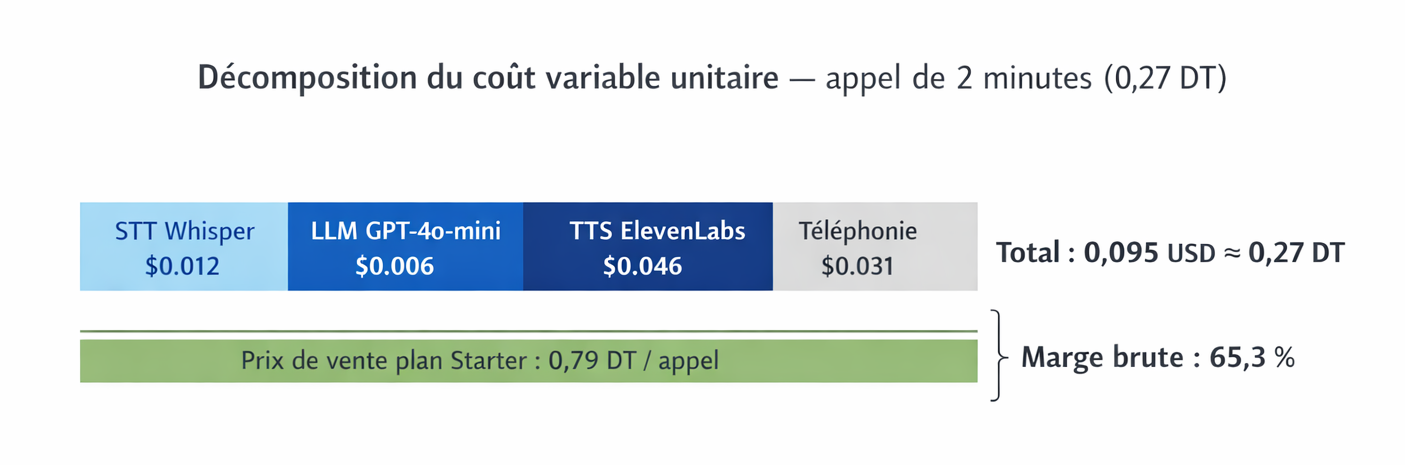
\includegraphics[width=0.92\textwidth]{figures/cout_variable_appel.png}
\caption{Décomposition du coût variable unitaire --- appel de 2 minutes (0,21 DT)}
\label{fig:cout_appel}
\end{figure}

%%%%%%%%%%%%%%%%%%%%%%%%%%%%%%%%%%%%%%%%%%%%%%%%%%%%%%%%%%%%%%%%%%%%%%%%%%%
\subsection{Business Model Canvas}
\label{section3.5.3}
%%%%%%%%%%%%%%%%%%%%%%%%%%%%%%%%%%%%%%%%%%%%%%%%%%%%%%%%%%%%%%%%%%%%%%%%%%%

Le Business Model Canvas (Osterwalder \& Pigneur, 2010) synthétise en une vue l'ensemble des décisions prises dans les sections précédentes --- segments, proposition de valeur, canaux, architecture de revenus --- et les confronte aux ressources, activités et partenariats nécessaires à l'exécution. L'enjeu n'est pas de remplir neuf cases, mais de vérifier que le modèle tient debout quand tous ses blocs sont mis en tension simultanément.

\begin{figure}[H]
    \centering
    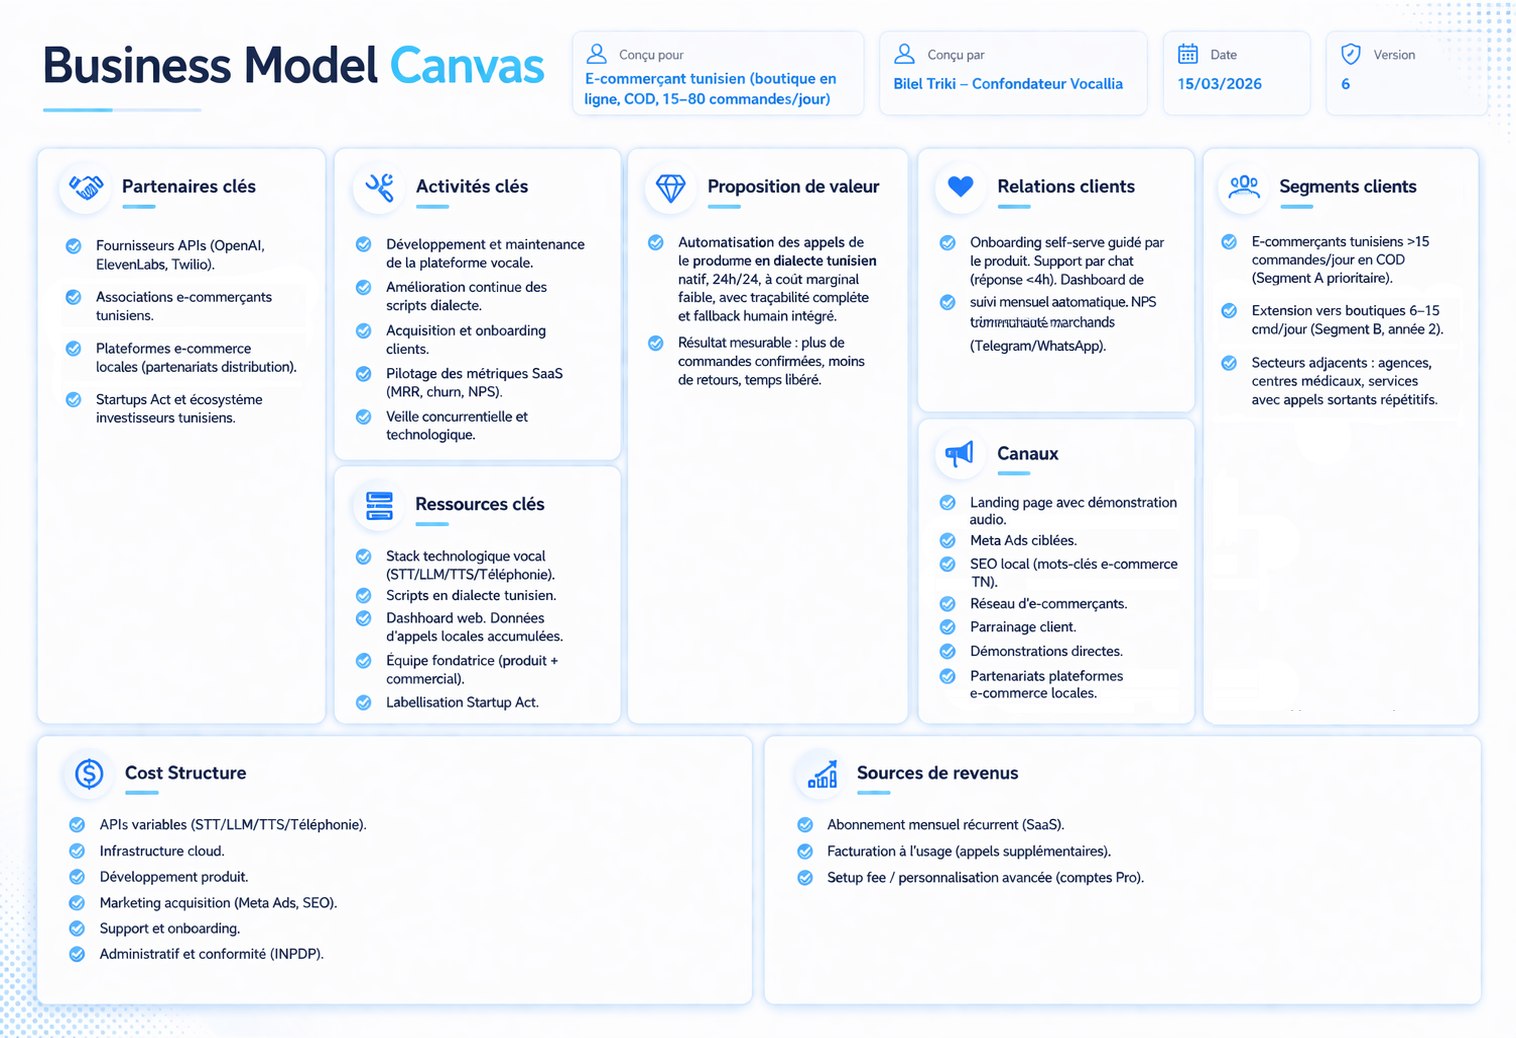
\includegraphics[width=\textwidth]{figures/bmc-vocallia.png}
    \caption{Business Model Canvas de Vocallia}
    \label{fig:bmc-vocallia}
\end{figure}

Les neuf blocs du BMC se résument comme suit. Les \textbf{segments de clientèle} ciblent en priorité les e-commerçants tunisiens à fort volume COD (Segment A), avec une extension vers les PME de services en année 2. La \textbf{proposition de valeur} repose sur l'automatisation des appels de confirmation en dialecte tunisien, avec dashboard de suivi intégré. Les \textbf{canaux} combinent vente directe B2B, acquisition digitale (Meta Ads, SEO) et réseau de partenaires. La \textbf{relation client} est conçue pour être majoritairement auto-gérée par le produit : onboarding guidé, démonstration personnalisée, suivi via tableau de bord. Les \textbf{sources de revenus} comprennent les abonnements mensuels (trois paliers), la facturation à l'usage et les frais d'intégration Pro. Les \textbf{ressources clés} sont l'infrastructure vocale, les modèles IA adaptés au dialecte tunisien, et les compétences en développement et intégration. Les \textbf{activités clés} couvrent le développement de la plateforme, l'amélioration continue des scripts, l'intégration e-commerce et l'acquisition client. Les \textbf{partenaires clés} --- OpenAI, ElevenLabs, Twilio --- sont gérés via une architecture multi-fournisseurs substituable. La \textbf{structure de coûts} est dominée par les variables (APIs), avec des coûts fixes limités à l'infrastructure cloud et au développement.

\medskip
\noindent\textbf{Lecture analytique du BMC.} Le modèle tient par un alignement fort entre trois blocs : la proposition de valeur répond à un problème structurel (confirmation COD), quotidien, et directement monétisable ; les canaux sont peu coûteux et empiriquement validés (CPL de 0,36~\euro{} en phase Muvaka) ; la relation client est conçue pour être auto-gérée par le produit, ce qui rend le modèle opérable avec une équipe de deux personnes en phase d'amorçage. La structure de coûts, dominée par les variables (APIs), confère au modèle sa propriété la plus précieuse : la scalabilité sans dégradation de marge. Le principal risque structurel est la concentration des partenaires clés --- trois fournisseurs d'APIs dont la défaillance ou la hausse tarifaire impacterait directement la rentabilité. L'architecture multi-fournisseurs, intégrée dès la conception, en est la réponse.

Le modèle étant structurellement viable, la section suivante en déploie les leviers opérationnels.

%%%%%%%%%%%%%%%%%%%%%%%%%%%%%%%%%%%%%%%%%%%%%%%%%%%%%%%%%%%%%%%%%%%%%%%%%%%
\section{Stratégie marketing opérationnelle --- cadre 8P}
\label{section3.6}
%%%%%%%%%%%%%%%%%%%%%%%%%%%%%%%%%%%%%%%%%%%%%%%%%%%%%%%%%%%%%%%%%%%%%%%%%%%

\subsection{Plan marketing opérationnel --- Marketing mix 8P}

Le plan marketing opérationnel de Vocallia s'articule autour du cadre élargi des
huit leviers du marketing mix (8P), développé à partir du modèle de
McCarthy (1960) et enrichi par Booms et Bitner (1981) pour les services.
Ce cadre structure les décisions opérationnelles de Vocallia selon trois
dimensions indissociables : la dimension technologique (solution SaaS), la
dimension de service (automatisation conversationnelle) et la dimension
relationnelle (accompagnement des e-commerçants tunisiens). Chaque levier
est décliné en décisions précises, actions concrètes et indicateurs mesurables.

% ------------------------------------------------------------
\subsubsection{Produit (\textit{Product}) --- Une infrastructure vocale intelligente,
pas un simple outil}
% ------------------------------------------------------------

\paragraph{Positionnement produit.}
Vocallia n'est pas un chatbot vocal générique. C'est une infrastructure
d'automatisation conversationnelle spécialisée, conçue pour un cas d'usage
précis --- la confirmation téléphonique des commandes e-commerce --- dans un
contexte linguistique spécifique, le dialecte tunisien avec code-switching
arabe/français. Cette spécialisation, cohérente avec le positionnement défini en
section~\ref{section3.2}, constitue le premier avantage concurrentiel défendable
du produit.

\paragraph{Architecture fonctionnelle.}
Le produit repose sur un pipeline vocal en cinq étapes séquentielles :
\begin{enumerate}
    \item \textbf{Déclenchement automatique} : à la réception d'une commande via
    webhook (Shopify, WooCommerce, API personnalisée), l'agent Vocallia initie
    l'appel sortant sans intervention humaine.
    \item \textbf{Reconnaissance vocale} (\textit{Speech-to-Text}) : conversion
    de la réponse du client en texte, via Whisper (OpenAI) avec ajustements pour
    le dialecte tunisien.
    \item \textbf{Compréhension et décision} (\textit{LLM}) : analyse de
    l'intention du client (confirmation, annulation, demande d'information,
    silence), génération de la réponse adaptée.
    \item \textbf{Synthèse vocale} (\textit{Text-to-Speech}) : conversion du
    texte généré en voix naturelle via ElevenLabs ou Azure Neural TTS.
    \item \textbf{Remontée des résultats} : mise à jour du statut de commande
    dans le système du marchand, notification en temps réel sur le tableau de bord.
\end{enumerate}

\paragraph{Offre produit structurée en trois paliers.}
La gamme est conçue selon une logique de \textit{good-better-best}, permettant à
chaque segment de trouver une entrée adaptée à son volume et à ses besoins :

\begin{itemize}
    \item \textbf{Plan Starter (79~DT/mois)} : 100~appels inclus, dialecte
    tunisien natif, dashboard de base, intégration webhook standard. Conçu pour
    les boutiques traitant 5 à 15~commandes par jour.
    \item \textbf{Plan Croissance (149~DT/mois)} : 300~appels inclus, dashboard
    complet avec export, rapports hebdomadaires automatiques, support prioritaire.
    Pour les boutiques à 15--50~commandes par jour.
    \item \textbf{Plan Pro (299~DT/mois)} : 800~appels inclus, intégration CRM
    avancée, scripts conversationnels personnalisés, rapport mensuel analytique,
    account manager dédié. Pour les structures à fort volume ($>$~50~commandes/jour).
\end{itemize}

\paragraph{Roadmap produit.}
Au-delà du cas d'usage initial (confirmation de commande), la feuille de route
produit prévoit l'extension vers d'autres scénarios conversationnels : relance
après abandon de panier (trimestre~3), rappel de rendez-vous pour les secteurs
de la santé et des services (année~2), qualification de leads entrants (année~2),
et service après-vente automatisé (année~3). Cette vision multi-cas d'usage
renforce la valeur à long terme du produit et réduit le risque de dépendance à
un unique segment.

\paragraph{Métriques produit.}
Les indicateurs de performance produit suivis sont : le taux de confirmation par
appel (objectif~$>$~70~\%), la durée moyenne d'appel (objectif~$<$~90~secondes),
la latence de réponse de l'agent (objectif~$<$~800~ms), le taux de déviation vers
un agent humain (objectif~$<$~15~\%), et le Net Promoter Score mensuel collecté
auprès des marchands (objectif~$>$~40).

% ------------------------------------------------------------
\subsubsection{Prix (\textit{Price}) --- Un pricing ancré sur la valeur créée,
pas sur les coûts}
% ------------------------------------------------------------

\paragraph{Philosophie tarifaire.}
La stratégie de prix de Vocallia est fondée sur la valeur créée pour le client,
et non sur une logique de coût majoré. Cette approche, recommandée pour les
startups SaaS B2B en phase d'amorçage (Anderson et al., \textit{Value-Based
Pricing}, 2010), permet de capturer une part de la valeur générée plutôt que
de se positionner sur la seule compétitivité tarifaire --- et donc de protéger
la marge à mesure que les coûts d'API diminuent.

\paragraph{Justification économique du pricing côté fournisseur.}
Le coût variable total d'un appel de deux minutes est estimé à environ 0,27~DT
(cf. figure~\ref{fig:cout_appel}). Sur cette base,
le plan Starter (79~DT pour 100~appels, soit 0,79~DT par appel) génère une marge
brute d'environ 65,3~\%. Ce niveau demeure élevé pour une offre SaaS en phase
d'amorçage, tout en préservant une structure de coûts compatible avec la scalabilité
du modèle.

\paragraph{Justification économique côté client.}
Pour un marchand traitant 150~commandes par mois avec un taux de retour de 15~\%
et un coût logistique de 12~DT par retour non anticipé, le coût mensuel
des retours s'élève à 270~DT. Si Vocallia réduit ce taux de 30~\% --- hypothèse
conservatrice basée sur l'amélioration du taux de joignabilité --- l'économie
mensuelle atteint 81~DT, soit davantage que le plan Starter (79~DT). L'abonnement
s'autofinance par la seule réduction des pertes logistiques, sans même comptabiliser
le temps opérationnel libéré pour le gérant.

\paragraph{Politique tarifaire complémentaire.}
En complément de l'abonnement mensuel, deux mécanismes tarifaires sont prévus :
\begin{itemize}
    \item \textbf{Appels supplémentaires} : facturation unitaire au-delà du
    forfait (0,90~DT/appel pour Starter, 0,70~DT pour Croissance, 0,50~DT pour
    Pro), alignant le coût marginal sur la valeur créée.
    \item \textbf{Setup fee} : frais uniques de configuration pour le plan Pro
    (500~DT), couvrant le paramétrage du CRM, la personnalisation des scripts et
    la formation initiale du marchand.
\end{itemize}

\paragraph{Pilote d'entrée sans engagement.}
Une offre d'entrée à risque nul complète le dispositif : 50~appels gratuits sur les vraies
commandes du client, sans carte bancaire requise. Ce mécanisme, inspiré du
modèle \textit{Product-Led Growth} (Wuebben, 2021), supprime la barrière
psychologique à l'entrée et permet au produit de se vendre lui-même avant
toute transaction commerciale.

% ------------------------------------------------------------
\subsubsection{Distribution (\textit{Place}) --- Un modèle 100~\% digital,
pensé pour une adoption sans friction}
% ------------------------------------------------------------

\paragraph{Canal unique : SaaS cloud.}
La distribution de Vocallia est entièrement dématérialisée. Il n'existe pas de
version physique du produit, pas de déplacement commercial requis, et pas
d'installation locale nécessaire dans la configuration standard. Cette approche
est cohérente avec le profil des clients cibles --- des e-commerçants actifs en
ligne --- et avec les contraintes budgétaires d'une startup en amorçage.

\paragraph{Parcours d'activation client.}
Le parcours complet d'un nouveau client se déroule en quatre étapes, toutes
réalisables sans contact humain :
\begin{enumerate}
    \item \textbf{Inscription} sur la landing page (email + numéro de téléphone),
    accès immédiat au pilote gratuit.
    \item \textbf{Configuration guidée} : assistant d'onboarding en 5~étapes
    pour connecter la source de commandes (webhook ou import CSV).
    \item \textbf{Activation} : premier appel envoyé automatiquement dès la
    réception d'une commande de test. Temps de mise en service cible~: moins de
    20~minutes.
    \item \textbf{Upgrade} : proposition automatique de passage au plan payant
    après consommation des 50~appels gratuits, avec affichage du résultat
    obtenu pendant le pilote.
\end{enumerate}

\paragraph{Déploiement géographique progressif.}
La stratégie de distribution suit une logique de concentration géographique
initiale, privilégiant les gouvernorats à forte densité de e-commerçants :
Grand Tunis (Tunis, Ariana, Ben Arous, Manouba) en priorité, suivi de Sfax et
Sousse en phase 2. Cette concentration permet d'optimiser les efforts de
support et de construire des effets de réseau locaux (bouche-à-oreille entre
marchands d'un même secteur géographique).

\paragraph{Option déploiement on-premise.}
Pour les secteurs sensibles (banque, santé, assurances), une option de
déploiement sur infrastructure privée est documentée et proposée sur devis.
Cette flexibilité architecturale répond aux exigences de souveraineté des
données et constitue un argument commercial différenciant pour les comptes Pro.

% ------------------------------------------------------------
\subsubsection{Communication (\textit{Promotion}) --- Une stratégie de preuve
à faible coût d'acquisition}
% ------------------------------------------------------------

\paragraph{Philosophie de communication.}
La stratégie de communication repose sur un principe central :
\textbf{montrer plutôt que promettre}. Dans un marché où la méfiance envers les
promesses technologiques est réelle, chaque canal est conçu comme un vecteur
de preuve concrète --- un extrait d'appel réel vaut plus que dix arguments.

\paragraph{Canal 1 --- Meta Ads (Facebook / Instagram).}
Les campagnes publicitaires Meta constituent le canal d'acquisition principal
en phase de lancement. Les données de la phase exploratoire Muvaka (avril~2025)
ont démontré la viabilité de ce canal : coût par lead de 0,36~\euro{} pour un budget
de 10~\euro{}, taux de clic de 10,9~\% sur la campagne Website Visit --- des résultats
significativement plus favorables que les benchmarks B2B habituels sur
Meta Ads (3--15~\euro{} par lead).

La stratégie publicitaire est structurée en trois phases~:
\begin{itemize}
    \item \textbf{Phase Teasing (semaines~1--2)} : vidéo courte (15~secondes)
    montrant un extrait d'appel IA en dialecte tunisien, sans révéler le produit.
    Objectif : générer la curiosité et mesurer l'engagement.
    \item \textbf{Phase Lancement (semaines~3--6)} : campagne Leads avec
    formulaire intégré proposant le pilote gratuit. Ciblage : e-commerçants
    tunisiens, 25--45~ans, intérêts e-commerce et business.
    \item \textbf{Phase Rétention (mois~2 et au-delà)} : retargeting des
    visiteurs non convertis, témoignages clients pilotes, contenu éducatif sur
    la valeur de l'automatisation vocale.
\end{itemize}

\paragraph{Canal 2 --- Content marketing et SEO local.}
Une stratégie de contenu éducatif est déployée sur deux supports~:
\begin{itemize}
    \item \textbf{Blog Vocallia} : articles optimisés pour le référencement
    naturel sur des requêtes spécifiques (exemples : \og{}automatiser les appels
    commande Tunisie\fg{}, \og{}réduire les retours colis e-commerce\fg{}, \og{}agent IA
    tunisien\fg{}). Objectif~: capter le trafic en phase de recherche active sans
    coût publicitaire.
    \item \textbf{Vidéos tutoriels} (YouTube / Facebook) : démonstrations
    pratiques de l'interface Vocallia, cas d'usage filmés avec de vrais marchands,
    FAQ en dialecte tunisien. Ces formats répondent aux objections les plus
    fréquentes identifiées dans l'étude terrain (\og{}est-ce que l'IA parle vraiment
    tunisien~?\fg{}, \og{}comment mes clients vont réagir~?\fg{}).
\end{itemize}

\paragraph{Canal 3 --- Démonstration directe.}
Le mécanisme de conversion le plus puissant est la démonstration en temps réel :
lors d'un premier contact, l'équipe déclenche un appel vers le téléphone du
prospect, simulant une confirmation de commande en dialecte tunisien. L'effet
de surprise et la naturalité de l'échange court-circuitent les objections
rationnelles --- c'est le moment de bascule identifié par les personas.

\paragraph{Canal 4 --- Programme de parrainage (\textit{referral}).}
Un mécanisme de recommandation structuré est mis en place dès le premier mois
d'activité~: tout client actif ayant recommandé Vocallia à un autre marchand
bénéficie d'un mois offert (valeur~: 79 à 299~DT selon son plan), et le filleul
reçoit son pilote étendu à 100~appels au lieu de 50. Ce mécanisme exploite la
dynamique communautaire des e-commerçants tunisiens, qui partagent activement
leurs pratiques opérationnelles dans des groupes Facebook et WhatsApp dédiés.

\paragraph{Canal 5 --- Partenariats éducatifs et institutionnels.}
Des partenariats sont développés avec les structures d'accompagnement des
entrepreneurs numériques tunisiens~: incubateurs (Flat6Labs, StartupBootcamp
Africa), associations d'e-commerçants, chambres de commerce régionales. Ces
partenariats permettent d'accéder à des audiences qualifiées sans coût
publicitaire direct et renforcent la crédibilité institutionnelle du projet.

% ------------------------------------------------------------
\subsubsection{Personnel (\textit{People}) --- Une équipe restreinte,
un produit qui assume le rôle commercial}
% ------------------------------------------------------------

\paragraph{Structure initiale de l'équipe.}
En cohérence avec le modèle \textit{Product-Led Growth} adopté, l'équipe
commerciale de Vocallia est volontairement restreinte en phase d'amorçage.
Le produit lui-même assume une grande partie du rôle commercial~: l'onboarding
est automatisé, la preuve de valeur est intégrée au pilote, et la
conversion est déclenchée par le dashboard de suivi des résultats.

L'équipe initiale se compose de~:
\begin{itemize}
    \item \textbf{Le porteur de projet} (CEO) : vision stratégique, développement
    commercial, gestion des partenariats, démonstrations directes auprès des
    prospects prioritaires.
    \item \textbf{Le co-fondateur technique} (CTO) : développement et maintenance
    du pipeline vocal, gestion des API, amélioration continue des modèles.
    \item \textbf{Support client} (freelance ou temps partiel, à partir du
    mois~3) : onboarding des nouveaux clients, réponse aux questions techniques,
    suivi des comptes Pro.
\end{itemize}

\paragraph{Formation et qualité de service.}
L'ensemble de l'équipe est formé sur les spécificités de la relation client
B2B dans le contexte tunisien~: compréhension des cycles de décision des PME,
maîtrise des objections liées à l'IA vocale, capacité à réaliser une
démonstration produit en conditions réelles. Un guide de vente interne est
rédigé et mis à jour mensuellement, intégrant les nouvelles objections rencontrées
sur le terrain et les réponses les plus efficaces.

\paragraph{Évolution de l'équipe.}
La croissance de l'équipe est conditionnée à l'atteinte des jalons commerciaux~:
recrutement d'un commercial terrain au-delà de 50~clients actifs, recrutement
d'un chargé de \textit{customer success} au-delà de 100~clients actifs.

% ------------------------------------------------------------
\subsubsection{Processus (\textit{Process}) --- Minimiser le délai entre
la découverte et la première preuve de valeur}
% ------------------------------------------------------------

\paragraph{Cartographie du parcours client.}
Le processus client de Vocallia est conçu pour minimiser le \textit{Time to Value}
(TTV) --- le délai entre la découverte du produit et la première preuve de valeur
perçue par le client. Cet indicateur est critique pour la rétention~: plus il
est court, plus le taux de conversion du pilote vers le plan payant est élevé
(OpenView Partners, \textit{PLG Benchmark}, 2024).

Le parcours se décompose en sept étapes mesurées~:

\begin{enumerate}
    \item \textbf{Découverte} (publicité, bouche-à-oreille, SEO) $\rightarrow$ atterrissage
    sur la landing page.
    \item \textbf{Inscription} (email + téléphone) $\rightarrow$ accès immédiat au tableau
    de bord. Durée cible~: moins de 2~minutes.
    \item \textbf{Configuration} (connexion de la source de commandes)
    $\rightarrow$ assistant guidé en 5~étapes. Durée cible~: moins de 15~minutes.
    \item \textbf{Premier appel} $\rightarrow$ déclenché automatiquement sur la prochaine
    commande reçue. Durée cible depuis l'inscription~: moins de 24~heures.
    \item \textbf{Consultation du tableau de bord} $\rightarrow$ visualisation des résultats.
    Premier signal de rétention~: le client revient consulter son dashboard.
    \item \textbf{Consommation du pilote} (50~appels) $\rightarrow$ proposition automatique
    d'upgrade avec affichage des résultats obtenus.
    \item \textbf{Conversion payante} $\rightarrow$ choix du plan adapté au volume, activation
    de la facturation.
\end{enumerate}

\paragraph{Gestion des cas d'erreur.}
Tout scénario d'appel qui dépasse les capacités de l'agent IA déclenche
automatiquement une notification au marchand (SMS + notification dashboard) avec
le détail de l'échange et la recommandation d'un rappel humain. Ce mécanisme
de \textit{graceful fallback} garantit qu'aucune commande n'est perdue en cas
de limitation de l'IA et renforce la confiance du marchand dans le système.

\paragraph{Processus d'amélioration continue.}
Les transcriptions d'appels (anonymisées, avec consentement) alimentent un
cycle d'amélioration mensuel : identification des patterns d'échec, mise à jour
des scripts, test A/B sur un sous-ensemble de clients. Ce processus crée un
avantage cumulatif --- chaque appel enrichit le corpus local --- que les
concurrents entrants ne pourront pas répliquer instantanément.

% ------------------------------------------------------------
\subsubsection{Preuves physiques (\textit{Physical Evidence}) --- Rendre
visible et mesurable la valeur créée}
% ------------------------------------------------------------

\paragraph{Le défi des services immatériels.}
L'un des défis fondamentaux de la commercialisation d'un service IA est son
caractère immatériel : le client ne voit pas l'agent travailler, il ne perçoit
que les résultats. Les \textit{physical evidences} --- preuves tangibles de
la qualité du service --- jouent un rôle critique pour instaurer la
confiance (Zeithaml et al., \textit{Services Marketing}, 2018) et constituent
le mécanisme de rétention principal de Vocallia.

\paragraph{Tableau de bord comme preuve principale.}
Le dashboard Vocallia est conçu comme l'interface de confiance principale du
marchand. Il doit répondre à une question fondamentale en moins de 10~secondes~:
\og{}est-ce que Vocallia m'a été utile ce mois-ci~?\fg{} Pour cela, il affiche en
premier plan quatre indicateurs clés~: commandes confirmées automatiquement,
temps opérationnel libéré, retours potentiellement évités, et taux de
joignabilité des clients.

\paragraph{Rapport mensuel automatique.}
À la fin de chaque mois, un rapport synthétique est généré et envoyé par email
au marchand. Ce document d'une page présente les métriques clés du mois, la
comparaison avec le mois précédent, et une recommandation automatique
(augmenter le volume d'appels, étendre à d'autres cas d'usage, passer au palier
supérieur). Ce rapport crée un rendez-vous mensuel régulier entre Vocallia et
son client, renforçant l'ancrage de la solution dans les habitudes opérationnelles
et réduisant le risque de churn passif.

\paragraph{Transcriptions et enregistrements.}
Chaque appel génère une transcription consultable dans le tableau de bord.
Le marchand peut écouter l'appel, lire la transcription et vérifier que l'échange
a été conduit conformément à ses attentes. Cette transparence totale est à la
fois une preuve de qualité et un outil d'ajustement~: si le marchand identifie
une formulation inadaptée, il peut la signaler et demander une mise à jour du script.

% ------------------------------------------------------------
\subsubsection{Partenariats (\textit{Partners}) --- Construire un écosystème
de crédibilité et d'accès}
% ------------------------------------------------------------

\paragraph{Partenaires technologiques.}
Les partenaires technologiques de Vocallia sont les fournisseurs d'API qui
constituent le pipeline vocal~: OpenAI (Whisper et GPT-4o-mini), ElevenLabs
(synthèse vocale), Twilio (téléphonie). Ces partenariats sont gérés selon une
architecture multi-fournisseurs permettant la substitution rapide d'un provider
en cas de hausse tarifaire ou d'interruption de service, limitant la
dépendance stratégique identifiée dans l'analyse SWOT.

\paragraph{Partenaires commerciaux.}
Deux catégories de partenaires commerciaux sont ciblées~:
\begin{itemize}
    \item \textbf{Plateformes e-commerce locales} (agrégateurs de boutiques
    tunisiennes, prestataires de logistique e-commerce) qui peuvent référencer
    Vocallia comme solution complémentaire. Un accord de \textit{referral} est
    proposé~: commission de 15~\% sur la première année de chaque client apporté.
    \item \textbf{Agences digitales et consultants} accompagnant des e-commerçants
    tunisiens dans leur transformation numérique. Ces intermédiaires ont une
    relation de confiance avec les marchands et peuvent recommander Vocallia
    dans le cadre d'une offre de service élargie.
\end{itemize}

\paragraph{Partenaires institutionnels.}
Des partenariats sont développés avec les structures d'appui à l'entrepreneuriat
numérique~: Startup Act (labellisation et accès aux avantages fiscaux),
incubateurs (Flat6Labs Tunisia, Cogite), associations professionnelles des
e-commerçants tunisiens. Ces partenariats renforcent la légitimité du projet
et ouvrent des accès à des réseaux qualifiés.

\paragraph{Tableau de synthèse --- plan marketing opérationnel 8P.}

\begin{figure}[H]
    \centering
    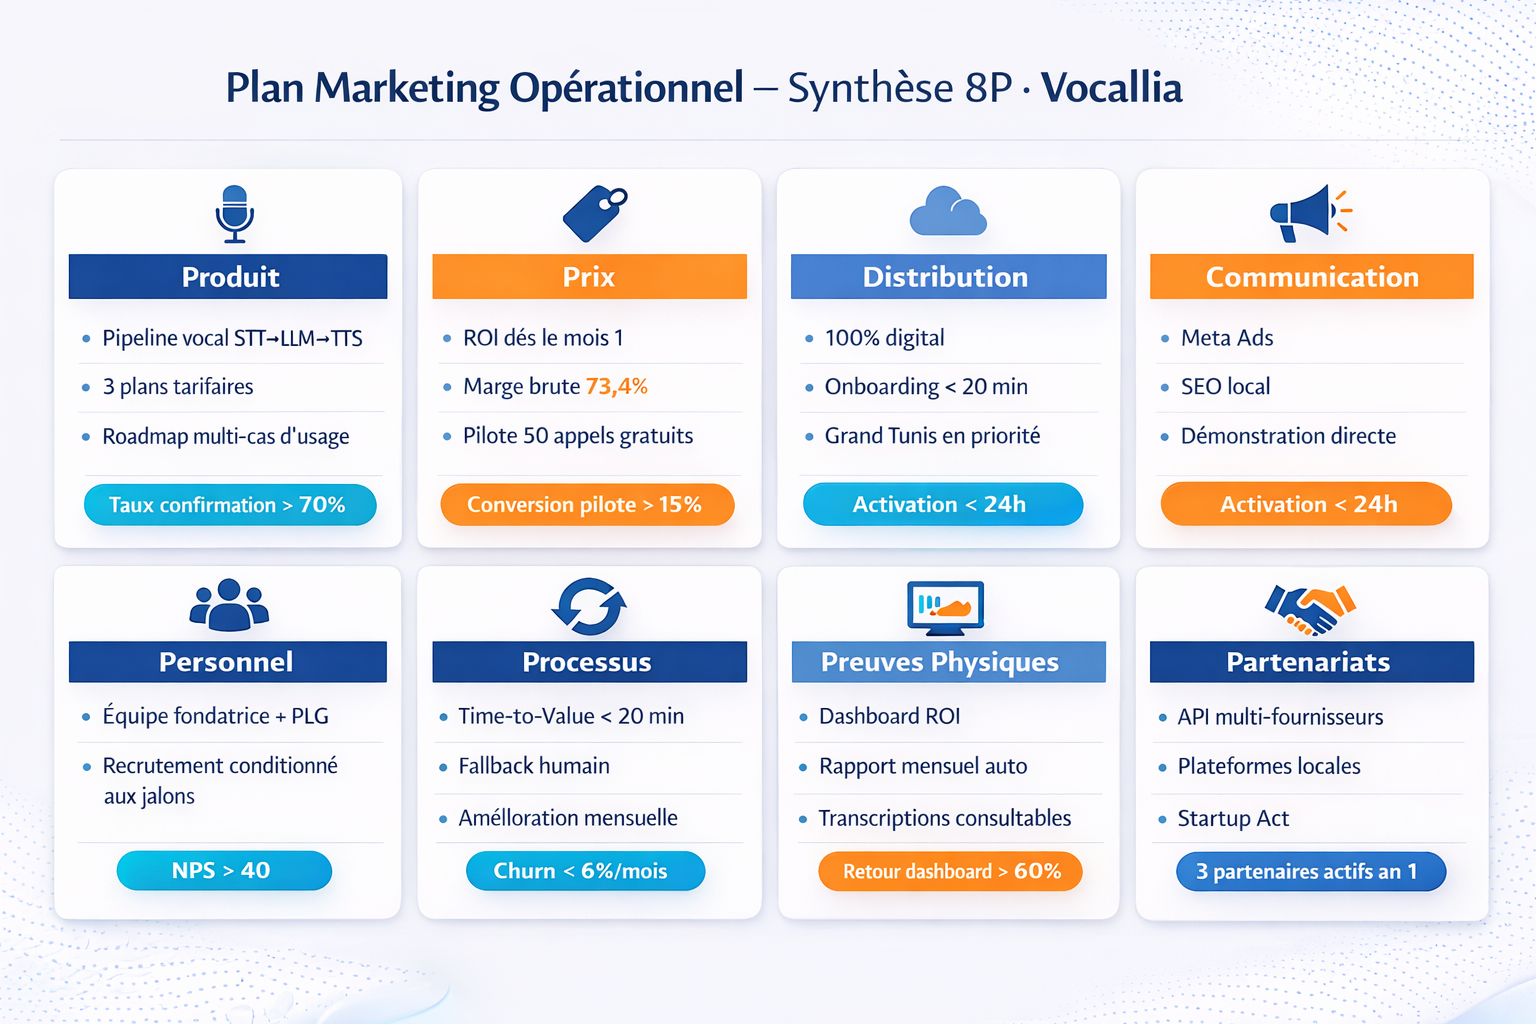
\includegraphics[width=\textwidth]{figures/marketing_8p_vocallia.png}
    \caption{Synthèse du plan marketing opérationnel Vocallia (8P)}
    \label{fig:marketing_8p}
\end{figure}

\medskip
Les huit leviers étant définis, la section suivante en organise le déploiement séquentiel à travers la stratégie go-to-market et le tunnel de conversion.

%%%%%%%%%%%%%%%%%%%%%%%%%%%%%%%%%%%%%%%%%%%%%%%%%%%%%%%%%%%%%%%%%%%%%%%%%%%
\section{Stratégie go-to-market et tunnel commercial}
\label{section3.7}
%%%%%%%%%%%%%%%%%%%%%%%%%%%%%%%%%%%%%%%%%%%%%%%%%%%%%%%%%%%%%%%%%%%%%%%%%%%

La stratégie go-to-market de Vocallia s'appuie sur le modèle Product-Led Growth (PLG), dans lequel le produit lui-même --- et non une force de vente --- constitue le principal vecteur d'acquisition, de conversion et de rétention. Ce modèle, adopté par 58~\% des entreprises B2B SaaS en 2024 (OpenView Partners, 2024), est le seul viable dans le contexte de Vocallia : budget marketing limité, marché de PME qui exigent une preuve avant tout engagement, et nécessité de convertir rapidement les marchands du Segment A pour atteindre le seuil de rentabilité identifié dans les projections.

%%%%%%%%%%%%%%%%%%%%%%%%%%%%%%%%%%%%%%%%%%%%%%%%%%%%%%%%%%%%%%%%%%%%%%%%%%%
\subsection{Entonnoir de conversion PLG}
\label{section3.7.1}
%%%%%%%%%%%%%%%%%%%%%%%%%%%%%%%%%%%%%%%%%%%%%%%%%%%%%%%%%%%%%%%%%%%%%%%%%%%

\begin{table}[H]
\centering
\caption{Entonnoir de conversion PLG --- Vocallia}
\vspace{4pt}
\begin{tabularx}{\textwidth}{|>{\raggedright\arraybackslash}p{2cm}|>{\raggedright\arraybackslash}X|>{\raggedright\arraybackslash}X|>{\raggedright\arraybackslash}p{2.2cm}|}
\hline
\textbf{Étape} & \textbf{Mécanisme} & \textbf{Objectif} & \textbf{KPI cible} \\
\hline
Découverte & Meta Ads ciblées (e-commerçants TN), SEO local, bouche à oreille réseau & Générer des leads qualifiés à faible coût & CPL $<$ 5 DT \\
\hline
Intérêt & Landing page avec démonstration audio d'un appel réel en dialecte tunisien & Créer le déclic \og{}ça marche vraiment en tunisien\fg{} & Conv. LP $>$ 8~\% \\
\hline
Activation & 50 appels gratuits sans engagement sur les vraies commandes du client & Prouver la valeur sur données réelles & Activation $>$ 70~\% \\
\hline
Conversion & Dashboard affichant les résultats chiffrés du pilote en DT & Transformer les données en décision d'achat & Free-to-paid $>$ 15~\% \\
\hline
Rétention & Rapport mensuel automatique, NPS, amélioration continue des scripts & Ancrer l'usage et réduire le churn & Churn mensuel $<$ 6~\% \\
\hline
Expansion & Upsell vers palier supérieur si volume dépassé. Recommandation à d'autres marchands. & Croître via les clients existants & NRR $>$ 110~\% \\
\hline
\end{tabularx}
\end{table}


%%%%%%%%%%%%%%%%%%%%%%%%%%%%%%%%%%%%%%%%%%%%%%%%%%%%%%%%%%%%%%%%%%%%%%%%%%%
\subsection{Tunnel commercial détaillé}
\label{section3.7.2}
%%%%%%%%%%%%%%%%%%%%%%%%%%%%%%%%%%%%%%%%%%%%%%%%%%%%%%%%%%%%%%%%%%%%%%%%%%%

L'entonnoir PLG se déploie opérationnellement en un tunnel commercial en six phases, chacune conçue pour réduire l'incertitude du marchand à chaque étape et le rapprocher de la conversion par les faits, pas par le discours.

\textbf{Phase 1 --- Prospection.} Identification des e-commerçants actifs à fort volume COD via Meta Ads, groupes Facebook e-commerce tunisiens, réseaux professionnels locaux. Critères de qualification : $>$15 commandes/jour, COD dominant, gérant joignable. Objectif : 20 à 30 leads qualifiés par mois en régime de croisière.

\textbf{Phase 2 --- Qualification.} Contact initial par message personnalisé, avec une question d'accroche centrée sur le problème : \og{}Combien de commandes perdez-vous par semaine faute d'avoir pu rappeler à temps ?\fg{}. Le taux de réponse à ce type de message orienté problème est supérieur à un discours centré sur les fonctionnalités.

\textbf{Phase 3 --- Démonstration.} Envoi d'un lien vers la landing page avec échantillon audio. Option : simulation en direct de 15 minutes sur un script adapté au profil du marchand. C'est le point de bascule --- en quelques secondes, la naturalité de la voix en dialecte tunisien dissipe les objections.

\textbf{Phase 4 --- Pilote.} Activation des 50 appels gratuits. Le marchand fournit ses premières commandes du jour. Vocallia confirme en automatique. Le fondateur reste disponible pour un suivi quotidien pendant les 7 premiers jours.

\textbf{Phase 5 --- Closing.} Présentation du dashboard à la fin du pilote : appels effectués, taux de confirmation, économies estimées en DT. La conversion est déclenchée par les chiffres du client lui-même. Proposition du plan adapté au volume observé.

\textbf{Phase 6 --- Onboarding et expansion.} Configuration complète des scripts, intégration CRM si applicable, formation au dashboard. À 90 jours, déclenchement de la demande de témoignage et de recommandation. À 6 mois, analyse de la montée en charge et proposition d'upsell vers le palier supérieur.

\medskip
La stratégie go-to-market étant définie, les sections suivantes en vérifient la viabilité financière. C'est ici que la démonstration de viabilité commerciale atteint son point culminant : la politique tarifaire prouve que le pricing est simultanément attractif et rentable ; les unit economics prouvent que le modèle d'acquisition est soutenable à l'échelle ; les projections financières prouvent que l'ensemble converge vers la rentabilité dans un délai maîtrisé.

%%%%%%%%%%%%%%%%%%%%%%%%%%%%%%%%%%%%%%%%%%%%%%%%%%%%%%%%%%%%%%%%%%%%%%%%%%%
\section{Stratégie de tarification}
\label{section3.8}
%%%%%%%%%%%%%%%%%%%%%%%%%%%%%%%%%%%%%%%%%%%%%%%%%%%%%%%%%%%%%%%%%%%%%%%%%%%

La politique de prix est le point de convergence de toute la stratégie commerciale : c'est elle qui traduit la proposition de valeur en transaction et qui détermine si le modèle est simultanément attractif pour le client, rentable pour Vocallia, et crédible face aux investisseurs. Le pricing est construit à partir de trois contraintes simultanées : la sensibilité prix déclarée sur le terrain, le coût unitaire réel par appel, et les ratios de référence de l'industrie SaaS. Ce triple ancrage élimine le risque d'un pricing arbitraire.

%%%%%%%%%%%%%%%%%%%%%%%%%%%%%%%%%%%%%%%%%%%%%%%%%%%%%%%%%%%%%%%%%%%%%%%%%%%
\subsection{Grille tarifaire --- trois paliers}
\label{section3.8.1}
%%%%%%%%%%%%%%%%%%%%%%%%%%%%%%%%%%%%%%%%%%%%%%%%%%%%%%%%%%%%%%%%%%%%%%%%%%%

\begin{table}[H]
\centering
\caption{Grille tarifaire Vocallia --- trois paliers}
\vspace{4pt}
\begin{tabularx}{\textwidth}{|>{\raggedright\arraybackslash}p{3.2cm}|>{\raggedright\arraybackslash}X|>{\raggedright\arraybackslash}X|>{\raggedright\arraybackslash}X|}
\hline
& \textbf{Starter} & \textbf{Croissance} & \textbf{Pro} \\
\hline
Prix mensuel & \textbf{79 DT} & \textbf{149 DT} & \textbf{299 DT} \\
\hline
Appels inclus/mois & 100 appels & 300 appels & 800 appels \\
\hline
Appel supplémentaire & 0,90 DT/appel & 0,70 DT/appel & 0,50 DT/appel \\
\hline
Dialecte tunisien & Oui & Oui & Oui \\
\hline
Dashboard & Basique & Complet & Complet $+$ export CSV \\
\hline
Intégration CRM & Non & Via webhook & Via webhook $+$ support dédié \\
\hline
Setup fee & Offert & Offert & 500 DT (unique) \\
\hline
Profil cible & Boutiques 5--15 cmd/jour & Boutiques 15--50 cmd/jour & Boutiques $>$50 cmd/jour \\
\hline
\end{tabularx}
\end{table}


%%%%%%%%%%%%%%%%%%%%%%%%%%%%%%%%%%%%%%%%%%%%%%%%%%%%%%%%%%%%%%%%%%%%%%%%%%%
\subsection{Justification économique du pricing}
\label{section3.8.2}
%%%%%%%%%%%%%%%%%%%%%%%%%%%%%%%%%%%%%%%%%%%%%%%%%%%%%%%%%%%%%%%%%%%%%%%%%%%

\noindent\textbf{Côté fournisseur --- marge brute.} Pour le plan Starter (79 DT / 100 appels) : coût variable $=$ 100 $\times$ 0,21 DT $=$ 21 DT. Marge brute $=$ 58 DT, soit \textbf{73,4~\%} --- au-dessus du seuil de référence SaaS de 70~\% (Bessemer Venture Partners, State of the Cloud, 2024). Pour le plan Croissance (149 DT / 300 appels) : coût variable $=$ 63 DT. Marge brute $=$ 86 DT, soit \textbf{57,7~\%}, compensée par le volume supérieur et la moindre intensité de support par client. Le plan Pro (299 DT / 800 appels) atteint un coût variable de 168 DT et une marge brute de 43,8~\%, mais intègre le setup fee de 500 DT et la facturation des dépassements à 0,50 DT/appel, ce qui rétablit la rentabilité globale du compte. La marge brute pondérée du portefeuille, dominée par les plans Starter et Croissance en phase de lancement, se situe au-dessus de 65~\%.

\medskip
\noindent\textbf{Côté client --- valeur créée supérieure au coût.} Pour un marchand à 150 commandes/mois avec un taux de retour de 15~\% (12 DT par retour), une réduction de 30~\% du taux de retour génère une économie de 81 DT --- supérieure au plan Starter à 79 DT. L'abonnement s'autofinance par les seules économies logistiques, sans même comptabiliser les gains opérationnels indirects.

\begin{tcolorbox}[colback=gray!8, colframe=gray!50, title=\textbf{Formule de valeur --- outil de closing commercial}, fonttitle=\bfseries]
\textbf{Économie mensuelle Vocallia} $=$ Commandes/mois $\times$ Taux de retour $\times$ Coût par retour $\times$ Taux de réduction attendu

\medskip
\textbf{Exemple :} 150 commandes $\times$ 15~\% $\times$ 12 DT $\times$ 30~\% $=$ \textbf{81 DT économisés/mois}

Plan Starter $=$ 79 DT/mois $\Rightarrow$ \textbf{L'abonnement s'autofinance dès le premier mois.}

\medskip
\noindent Cette formule est intégrée au dashboard et calculée automatiquement sur les données réelles du client pendant le pilote. C'est elle --- et non un argumentaire commercial --- qui déclenche la conversion.
\end{tcolorbox}

%%%%%%%%%%%%%%%%%%%%%%%%%%%%%%%%%%%%%%%%%%%%%%%%%%%%%%%%%%%%%%%%%%%%%%%%%%%
\section{Unit economics SaaS --- viabilité financière du modèle}
\label{section3.9}
%%%%%%%%%%%%%%%%%%%%%%%%%%%%%%%%%%%%%%%%%%%%%%%%%%%%%%%%%%%%%%%%%%%%%%%%%%%

Les unit economics sont le test décisif de la viabilité d'un modèle SaaS : ils répondent à une question simple --- chaque client acquis génère-t-il davantage de valeur qu'il n'en coûte à conquérir et à servir~? La politique tarifaire a établi que la marge brute dépasse 65~\% en pondéré. Cette section vérifie que cette marge se traduit en un modèle d'acquisition soutenable à l'échelle --- et fournit les métriques que tout investisseur examinera en premier.

%%%%%%%%%%%%%%%%%%%%%%%%%%%%%%%%%%%%%%%%%%%%%%%%%%%%%%%%%%%%%%%%%%%%%%%%%%%
\subsection{Calcul des métriques clés}
\label{section3.9.1}
%%%%%%%%%%%%%%%%%%%%%%%%%%%%%%%%%%%%%%%%%%%%%%%%%%%%%%%%%%%%%%%%%%%%%%%%%%%

\begin{table}[H]
\centering
\caption{Unit economics SaaS --- métriques clés Vocallia (scénario réaliste)}
\vspace{4pt}
\begin{tabularx}{\textwidth}{|>{\raggedright\arraybackslash}p{2.3cm}|>{\raggedright\arraybackslash}X|>{\raggedright\arraybackslash}p{2.5cm}|>{\raggedright\arraybackslash}X|}
\hline
\textbf{Métrique} & \textbf{Définition} & \textbf{Valeur cible} & \textbf{Base de calcul} \\
\hline
ARPU & Revenu moyen mensuel par client actif & 120 DT/mois & Mix des 3 paliers, dominance plan Croissance \\
\hline
Churn mensuel & Taux d'attrition mensuel & 5 -- 8~\% & Benchmark SaaS B2B PME : 5--10~\%/mois \\
\hline
LTV & Valeur vie client (ARPU / churn) & 1\,500 -- 2\,400 DT & 120 / 0,08 à 120 / 0,05 \\
\hline
CAC & Coût d'acquisition d'un client payant & $<$ 150 DT & 0,36~\euro{}/lead $\times$ taux conv. 15~\% $\approx$ 2,4~\euro{}/client qualifié \\
\hline
Ratio LTV:CAC & Viabilité du modèle d'acquisition & 10:1 à 16:1 & Benchmark minimal SaaS : 3:1 \\
\hline
CAC Payback & Mois pour récupérer le CAC & $<$ 2 mois & CAC 150 DT / ARPU 120 DT \\
\hline
MRR cible An 1 & MRR en fin d'année 1 & 4\,800 -- 6\,000 DT & 40--50 clients $\times$ 120 DT \\
\hline
\end{tabularx}
\end{table}


\medskip
La figure~\ref{fig:ltv_cac} met en perspective le ratio LTV:CAC projeté de Vocallia par rapport aux benchmarks de référence de l'industrie SaaS.

\begin{figure}[H]
\centering
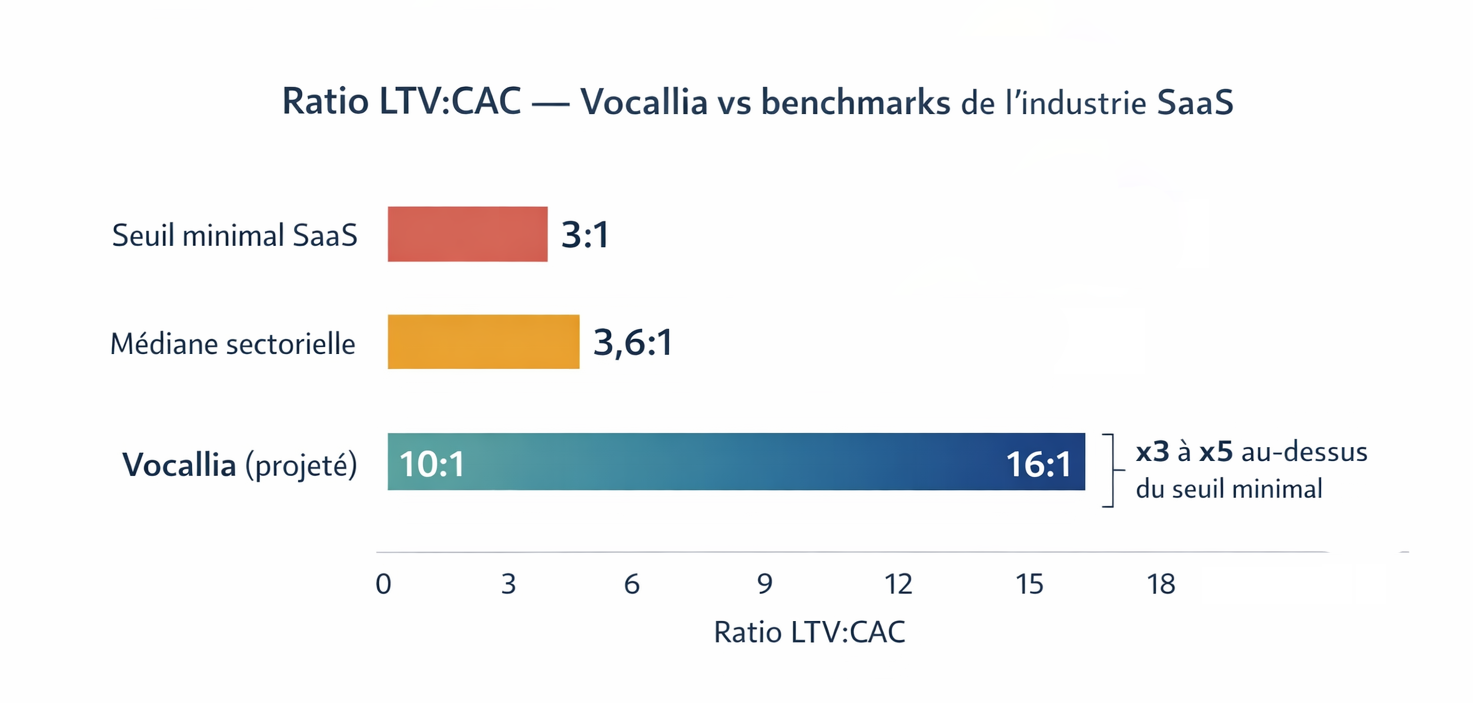
\includegraphics[width=0.92\textwidth]{figures/ltv_cac_benchmark.png}
\caption{Ratio LTV:CAC --- Vocallia vs benchmarks de l'industrie SaaS}
\label{fig:ltv_cac}
\end{figure}

\begin{tcolorbox}[colback=gray!8, colframe=gray!50, title=\textbf{Interprétation des unit economics}, fonttitle=\bfseries]
Un ratio LTV:CAC projeté entre 10:1 et 16:1 place Vocallia très au-dessus du seuil minimal de 3:1 recommandé par les investisseurs SaaS (Benchmarkit, 2024), et au-dessus de la médiane sectorielle de 3,6:1. Cette asymétrie repose sur deux caractéristiques structurelles du marché --- et non sur des hypothèses optimistes. Premièrement, le coût d'acquisition est empiriquement faible : le CPL de 0,36~\euro{} validé en phase Muvaka est 8 à 40 fois inférieur aux benchmarks B2B sur Meta Ads, un écart qui s'explique par la nouveauté de l'offre sur un marché sans concurrent direct. Deuxièmement, la valeur vie client est soutenue par un besoin non reportable : un e-commerçant en COD qui ne confirme pas ses commandes perd de l'argent chaque jour --- il n'a pas le luxe de suspendre son abonnement.

\medskip
Le facteur de risque principal est le churn. Une attrition mensuelle supérieure à 10~\% comprimerait la LTV sous 1\,200 DT et le ratio sous 8:1 --- encore viable, mais avec une marge de manœuvre réduite. C'est pourquoi le pilote gratuit, le dashboard et le rapport mensuel ne sont pas des fonctionnalités secondaires : ce sont les mécanismes de rétention qui protègent la LTV et, par conséquent, l'ensemble de l'économie du modèle.

\medskip
\noindent Ces métriques confirment que le modèle d'acquisition est financièrement soutenable. Les projections suivantes en vérifient la trajectoire sur trois ans.
\end{tcolorbox}

%%%%%%%%%%%%%%%%%%%%%%%%%%%%%%%%%%%%%%%%%%%%%%%%%%%%%%%%%%%%%%%%%%%%%%%%%%%
\section{Projections financières prévisionnelles --- trois scénarios}
\label{section3.10}
%%%%%%%%%%%%%%%%%%%%%%%%%%%%%%%%%%%%%%%%%%%%%%%%%%%%%%%%%%%%%%%%%%%%%%%%%%%

Les projections financières sont le dernier maillon de la chaîne de preuve : elles traduisent la segmentation, le pricing, les unit economics et le go-to-market en trajectoires de croissance chiffrées sur trente-six mois. Construites selon trois scénarios d'adoption (Maurya, 2012), elles permettent de vérifier que le modèle reste viable même dans l'hypothèse la plus conservatrice --- et d'identifier le seuil de clients actifs à partir duquel Vocallia devient rentable.

\medskip
\noindent\textbf{Hypothèses communes aux trois scénarios.} ARPU moyen de 120 DT/mois. Churn mensuel de 6~\%. Coût variable par appel de 0,21 DT. Charges fixes mensuelles : 1\,200 DT (an 1), 2\,000 DT (an 2), 3\,500 DT (an 3), reflétant une montée progressive des dépenses de structure avec la croissance.

%%%%%%%%%%%%%%%%%%%%%%%%%%%%%%%%%%%%%%%%%%%%%%%%%%%%%%%%%%%%%%%%%%%%%%%%%%%
\subsection{Tableau de projections sur 3 ans}
\label{section3.10.1}
%%%%%%%%%%%%%%%%%%%%%%%%%%%%%%%%%%%%%%%%%%%%%%%%%%%%%%%%%%%%%%%%%%%%%%%%%%%

\begin{table}[H]
\centering
\caption{Projections financières sur 3 ans --- trois scénarios Vocallia}
\vspace{4pt}
\begin{tabularx}{\textwidth}{|>{\raggedright\arraybackslash}p{3.8cm}|>{\raggedright\arraybackslash}X|>{\raggedright\arraybackslash}X|>{\raggedright\arraybackslash}X|}
\hline
\textbf{Indicateur} & \textbf{Scénario prudent} & \textbf{Scénario central} & \textbf{Scénario ambitieux} \\
\hline
\multicolumn{4}{|l|}{\textit{\textbf{Année 1}}} \\
\hline
Clients actifs (fin an 1) & 20 clients & 40 clients & 65 clients \\
MRR (fin an 1) & 2\,400 DT & 4\,800 DT & 7\,800 DT \\
CA annuel & $\sim$22\,000 DT & $\sim$45\,000 DT & $\sim$72\,000 DT \\
Résultat net & $-$8\,000 DT & $-$2\,000 DT & $+$14\,000 DT \\
\hline
\multicolumn{4}{|l|}{\textit{\textbf{Année 2}}} \\
\hline
Clients actifs (fin an 2) & 35 clients & 70 clients & 120 clients \\
MRR (fin an 2) & 4\,200 DT & 8\,400 DT & 14\,400 DT \\
CA annuel & $\sim$40\,000 DT & $\sim$80\,000 DT & $\sim$140\,000 DT \\
Résultat net & $-$3\,000 DT & $+$16\,000 DT & $+$56\,000 DT \\
\hline
\multicolumn{4}{|l|}{\textit{\textbf{Année 3}}} \\
\hline
Clients actifs (fin an 3) & 50 clients & 100 clients & 180 clients \\
MRR (fin an 3) & 6\,000 DT & 12\,000 DT & 21\,600 DT \\
CA annuel & $\sim$60\,000 DT & $\sim$120\,000 DT & $\sim$220\,000 DT \\
Résultat net & $+$9\,000 DT & $+$48\,000 DT & $+$128\,000 DT \\
\hline
\textbf{Seuil de rentabilité} & \textbf{An 3 --- T1} & \textbf{An 2 --- T3} & \textbf{An 1 --- T4} \\
\hline
\end{tabularx}
\end{table}


\medskip
La figure~\ref{fig:mrr_evolution} illustre la trajectoire du MRR pour chacun des trois scénarios, avec le seuil de rentabilité opérationnelle matérialisé.

\begin{figure}[H]
\centering
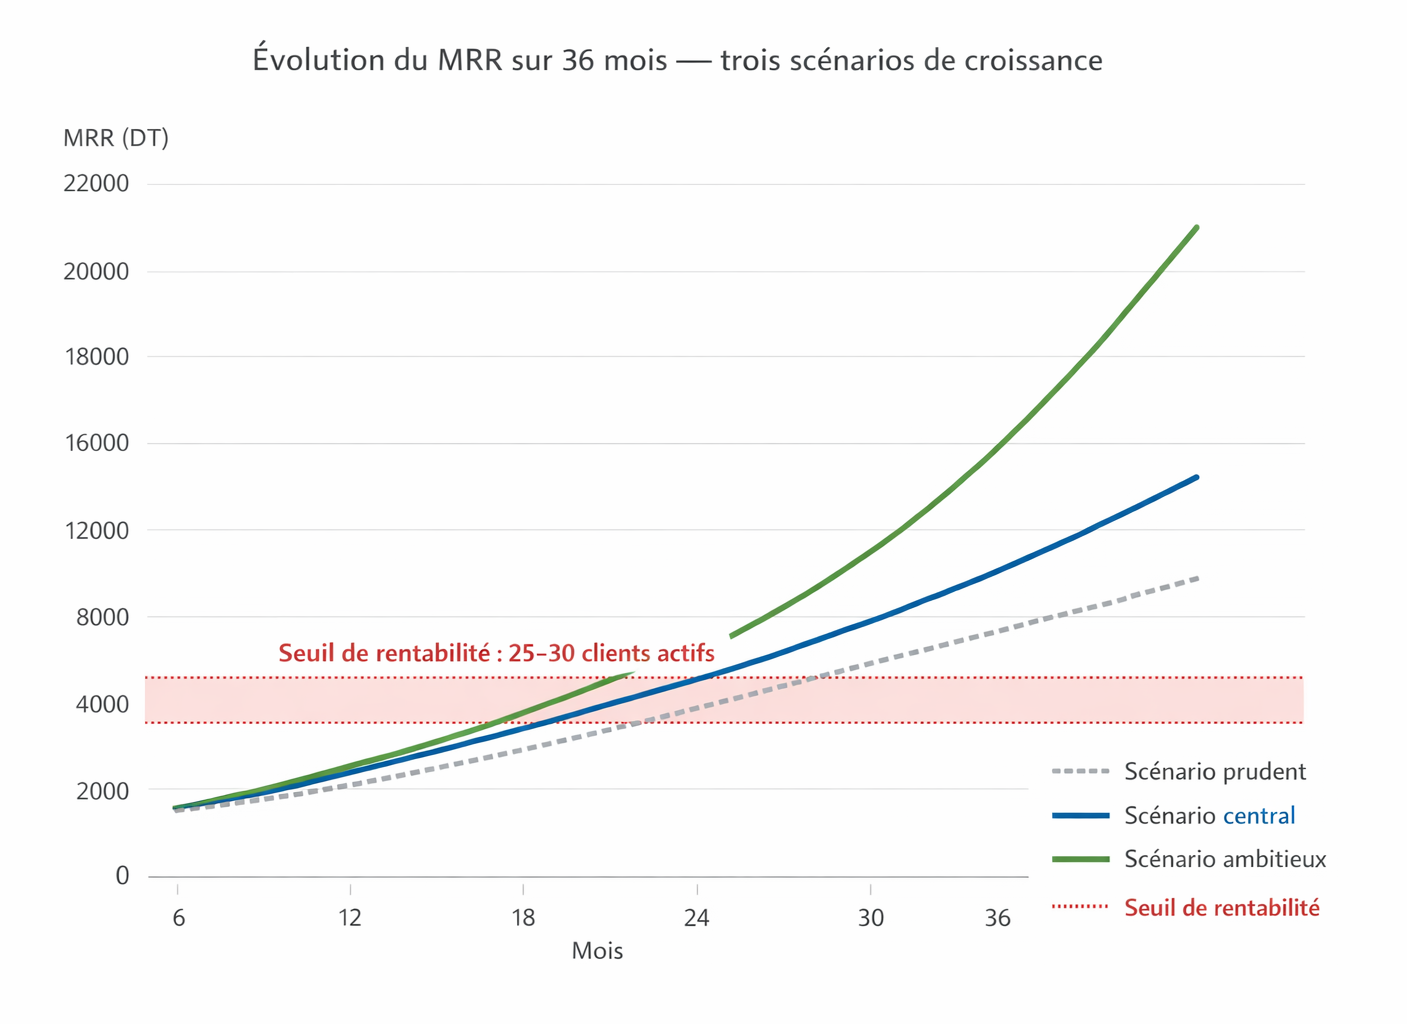
\includegraphics[width=\textwidth]{figures/mrr_evolution_36mois.png}
\caption{Évolution du MRR sur 36 mois --- trois scénarios de croissance}
\label{fig:mrr_evolution}
\end{figure}

%%%%%%%%%%%%%%%%%%%%%%%%%%%%%%%%%%%%%%%%%%%%%%%%%%%%%%%%%%%%%%%%%%%%%%%%%%%
\subsection{Lecture stratégique des scénarios}
\label{section3.10.2}
%%%%%%%%%%%%%%%%%%%%%%%%%%%%%%%%%%%%%%%%%%%%%%%%%%%%%%%%%%%%%%%%%%%%%%%%%%%

Le \textbf{scénario prudent} (20 clients en an 1) correspond à un rythme d'acquisition de 1 à 2 nouveaux clients par mois, avec un churn non encore maîtrisé. La rentabilité n'est atteinte qu'en début d'année 3. Ce scénario reste viable à condition de maintenir les charges fixes sous contrôle strict et de ne pas recruter avant que le MRR couvre les coûts fixes. Il représente le plancher de survie --- le scénario dans lequel le projet ne meurt pas, mais ne décolle pas non plus.

Le \textbf{scénario central} (40 clients en an 1, 100 en an 3) est le scénario de référence. Il suppose un rythme de 3 à 4 nouveaux clients par mois, cohérent avec un budget Meta Ads de 500 DT/mois et un taux de conversion free-to-paid de 15~\%. La rentabilité est atteinte au troisième trimestre de l'année 2 et le MRR dépasse 12\,000 DT en fin d'année 3 --- un niveau qui permet le réinvestissement en produit et en équipe.

Le \textbf{scénario ambitieux} (65 clients en an 1) suppose une diffusion accélérée par le bouche-à-oreille dans le réseau des e-commerçants ou par un partenariat de distribution avec une plateforme locale. La rentabilité est atteinte dès le quatrième trimestre de l'année 1. Ce scénario n'est pas irréaliste : il requiert un taux de recommandation élevé et un NPS supérieur à 50, deux conditions atteignables si la qualité dialectale et la fiabilité du service sont au rendez-vous.

\begin{tcolorbox}[colback=gray!8, colframe=gray!50, title=\textbf{Seuil critique opérationnel}, fonttitle=\bfseries]
Dans tous les scénarios, le seuil de rentabilité mensuelle est atteint à partir de \textbf{25 à 30 clients actifs}, soit un MRR de 3\,000 à 3\,600 DT. Ce chiffre est la milestone absolue du projet : en deçà, Vocallia consomme de la trésorerie ; au-delà, elle génère du profit réinvestissable. Il justifie rétrospectivement chaque décision de la chaîne stratégique : la concentration sur le Segment A (cycle de vente court), le pilote gratuit (accélérateur d'activation), le modèle PLG (coût d'acquisition minimal), le pricing à 79 DT (zone de confort validée). Toutes ces décisions sont calibrées pour atteindre 25 clients actifs dans les 12 premiers mois --- un objectif que même le scénario prudent atteint avant le mois 18.
\end{tcolorbox}

%%%%%%%%%%%%%%%%%%%%%%%%%%%%%%%%%%%%%%%%%%%%%%%%%%%%%%%%%%%%%%%%%%%%%%%%%%%
\section{Facteurs d'adoption et obstacles commerciaux}
\label{section3.11}
%%%%%%%%%%%%%%%%%%%%%%%%%%%%%%%%%%%%%%%%%%%%%%%%%%%%%%%%%%%%%%%%%%%%%%%%%%%

L'adoption d'une solution IA vocale par des PME e-commerce tunisiennes ne suit pas une logique linéaire. Elle s'inscrit dans la courbe de diffusion des innovations de Rogers (1962) : innovateurs (2,5~\%), adopteurs précoces (13,5~\%), majorité précoce (34~\%), majorité tardive (34~\%), retardataires (16~\%). La stratégie de Vocallia vise d'abord les adopteurs précoces --- profil Segment A --- avant de traverser le \og{}gouffre\fg{} vers la majorité précoce. Le tableau suivant identifie chaque facteur d'adoption ou de résistance et y associe la réponse stratégique déployée dans les sections précédentes.

\begin{table}[H]
\centering
\caption{Facteurs d'adoption et obstacles commerciaux --- Vocallia}
\vspace{4pt}
\begin{tabularx}{\textwidth}{|>{\raggedright\arraybackslash}p{3cm}|>{\raggedright\arraybackslash}p{1.8cm}|>{\raggedright\arraybackslash}p{1.5cm}|>{\raggedright\arraybackslash}X|}
\hline
\textbf{Facteur} & \textbf{Nature} & \textbf{Impact} & \textbf{Réponse stratégique} \\
\hline
Autofinancement visible dès le 1er mois & Accélérateur & Élevé & Formule de valeur chiffrée intégrée au dashboard, calculée sur données réelles \\
\hline
Naturalité du dialecte tunisien & Accélérateur & Très élevé & Démonstration audio sur appel réel avant tout engagement commercial \\
\hline
Pilote sans engagement financier & Accélérateur & Élevé & 50 appels gratuits : suppression totale du risque perçu à l'entrée \\
\hline
Références clients locales publiées & Accélérateur & Moyen & Recruter 3--5 ambassadeurs pilotes dès le lancement, avec témoignages vidéo \\
\hline
Résistance au changement (appel humain habituel) & Frein & Élevé & Démonstration comparative IA vs appel humain sur même script, métriques à l'appui \\
\hline
Crainte que l'IA soit mal perçue par les clients finaux & Frein & Moyen & Transparence dans les scripts + statistiques de satisfaction client post-appel \\
\hline
Sensibilité prix des PME tunisiennes & Frein & Élevé & Plan Starter à 79 DT aligné sur la zone de confort terrain. Pilote gratuit. \\
\hline
Absence de référence au lancement & Frein & Moyen & Partenariat 5 marchands pilotes avec études de cas publiées sur le site \\
\hline
Dépendance à la qualité du dialecte & Risque & Élevé & Amélioration continue des scripts, fine-tuning des prompts, boucle de feedback client \\
\hline
\end{tabularx}
\end{table}

%%%%%%%%%%%%%%%%%%%%%%%%%%%%%%%%%%%%%%%%%%%%%%%%%%%%%%%%%%%%%%%%%%%%%%%%%%%
\section{Conclusion}
\label{conclusion3}
%%%%%%%%%%%%%%%%%%%%%%%%%%%%%%%%%%%%%%%%%%%%%%%%%%%%%%%%%%%%%%%%%%%%%%%%%%%

Ce chapitre a construit la viabilité commerciale de Vocallia selon une chaîne stratégique où chaque décision découle de la précédente et en renforce la suivante. Quatre conclusions s'imposent.

\textbf{Le modèle est monétisable maintenant.} Le Segment A --- e-commerçants tunisiens à fort volume COD --- subit une douleur quotidienne et coûteuse à laquelle aucune solution locale ne répond. Le positionnement, la proposition de valeur et le pricing ont été calibrés sur ce segment. L'abonnement Starter à 79 DT génère une marge brute de 73,4~\% côté fournisseur et s'autofinance côté client, et 63,6~\% des répondants terrain acceptent un prix dans cette zone. La monétisation ne dépend pas d'une éducation du marché : le besoin est structurel et le client le sait.

\textbf{Le modèle scale.} Une marge brute pondérée supérieure à 65~\%, une structure de coûts dominée par les variables, et un modèle hybride abonnement/usage qui aligne revenus et valeur créée. Chaque client supplémentaire améliore la marge sans augmenter les coûts fixes. Le ratio LTV:CAC entre 10:1 et 16:1 --- avec un CAC payback inférieur à 2 mois et un coût d'acquisition 8 à 40 fois inférieur aux benchmarks sectoriels --- confirme que le modèle d'acquisition est soutenable bien au-delà du marché tunisien initial.

\textbf{Le modèle est défendable.} La barrière linguistique (dialecte tunisien natif + code-switching) offre une fenêtre d'avance de 18 à 36 mois. Chaque client actif enrichit le corpus de données d'appels locales, chaque mois d'usage augmente les coûts de migration vers un concurrent, et le réseau de témoignages se densifie. La défendabilité n'est pas statique : elle se renforce avec le temps.

\textbf{L'exécution est réaliste.} Le seuil de rentabilité opérationnelle --- 25 à 30 clients --- est atteignable dans les 12 à 18 premiers mois avec le modèle PLG déployé. Même dans le scénario le plus conservateur, le projet atteint l'équilibre en début d'année 3. Dans le scénario central, le MRR dépasse 12\,000 DT en fin d'année 3, ouvrant la voie au réinvestissement en produit et en expansion géographique.

\begin{quote}
\textit{Le chapitre suivant examinera la viabilité technique de Vocallia : architecture vocale, stack technologique, flux d'appel, latence, gestion des cas limites, besoins fonctionnels et non-fonctionnels, et ressources nécessaires au déploiement opérationnel de la solution.}
\end{quote}